\documentclass{article}  % Define la clase del documento.

% Paquetes de idioma y codificación
\usepackage[utf8]{inputenc}
\usepackage[T1]{fontenc}
\usepackage[spanish]{babel}  % Ajusta el idioma del documento a español.
\usepackage{tabularx}  % Permite la creación de tablas con ancho ajustable.

% Paquete de geometría para configurar márgenes y tamaño de papel
\usepackage[letterpaper, margin=3cm]{geometry}

% Paquetes de tipografía
\usepackage{mathptmx}    % Usa Times New Roman como fuente.
\usepackage{microtype}   % Mejora la justificación del texto.

% Paquetes para manejo de colores y gráficos
\usepackage{xcolor}      % Define y utiliza colores.
\usepackage{graphicx}    % Permite la inserción de imágenes.
\usepackage{tikz}        % Creación de gráficos vectoriales.
\usepackage{amsfonts}


% Configuración de enlaces y referencias cruzadas
\usepackage{hyperref}
\hypersetup{
    colorlinks   = true,
    linkcolor    = darkblue,
    citecolor    = black,
    filecolor    = blue,
    urlcolor     = blue
}

\usepackage{media9} % Permite la inserción de multimedia.

% Paquetes para la mejora visual de tablas y figuras
\usepackage{booktabs}    % Para tablas de alta calidad.
\usepackage{float}       % Controla la posición de figuras y tablas.

% Paquete para la personalización de códigos fuente
\usepackage{listings}
\lstset{
    literate=
    {á}{{\'a}}1 {é}{{\'e}}1 {í}{{\'i}}1 {ó}{{\'o}}1 {ú}{{\'u}}1
    {Á}{{\'A}}1 {É}{{\'E}}1 {Í}{{\'I}}1 {Ó}{{\'O}}1 {Ú}{{\'U}}1
    {ñ}{{\~n}}1 {Ñ}{{\~N}}1 {ü}{{\"u}}1 {Ü}{{\"U}}1,
    backgroundcolor=\color{backcolour},
    commentstyle=\color{codegreen},
    keywordstyle=\color{codepurple},
    numberstyle=\tiny\color{codegray},
    stringstyle=\color{red},
    basicstyle=\ttfamily\small,
    breakatwhitespace=false,
    breaklines=true,
    captionpos=b,
    keepspaces=true,
    numbers=left,
    numbersep=5pt,
    showspaces=false,
    showstringspaces=false,
    showtabs=false,
    tabsize=2,
    language=TeX,
    morecomment=[l]\#,
    frame=single,
    rulecolor=\color{black}
}

% Definición de colores al estilo Visual Studio Code
\definecolor{darkblue}{rgb}{0.0, 0.0, 0.55}  % Enlaces
\definecolor{codegreen}{rgb}{0.25, 0.49, 0.48}  % Comentarios
\definecolor{codegray}{rgb}{0.5, 0.5, 0.5}  % Números y anotaciones
\definecolor{codepurple}{rgb}{0.58, 0, 0.82}  % Palabras clave
\definecolor{backcolour}{rgb}{0.95, 0.95, 0.92}  % Fondo de código

% Configuraciones de párrafo y matemáticas
\usepackage{amsmath}
\usepackage{parskip}    % Espaciado entre párrafos.
\usepackage{ragged2e}   % Justificación mejorada.

% Configuración de secciones y encabezados
\usepackage{titlesec}
\titleclass{\part}{top}
\titleformat{\part}[display]
  {\normalfont\huge\bfseries\centering}{\thepart}{40pt}{\Huge}
\titlespacing*{\part}{0pt}{-60pt}{10pt}
\titleformat{\part}
  {\normalfont\huge\bfseries}{}{0pt}{}
\titleformat{\part}[display]
  {\normalfont\huge\bfseries}{}{0pt}{}
  [\thispagestyle{fancy}]

% Encabezado y pie de página
\usepackage{fancyhdr}
\pagestyle{fancy}
\fancyhf{}
\fancyhead[L]{\raisebox{0.20cm}{\textbf{Dinamica Prueba 1}}}
\fancyhead[R]{\raisebox{0.1cm}{
\includegraphics[width=0.25\linewidth]{LOGO_UNIVERSIDAD.jpg}}}
\fancyhead[C]{\rule{\textwidth}{0.6pt}}
\fancyfoot[C]{\rule{\textwidth}{0.6pt}}
\fancyfoot[R]{\raisebox{-1.5\baselineskip}{\thepage}}
\renewcommand{\headrulewidth}{0pt}
\renewcommand{\footrulewidth}{0pt}

% Geometría avanzada
\geometry{
  top=3.5cm,
  bottom=2.5cm,
  headheight=2.5cm
}

% Bibliografía
\usepackage{natbib}
\bibliographystyle{unsrtnat}

\begin{document}

%---------------------------------------- PORTADA ----------------------------------------
\begin{titlepage}
\newcommand{\HRule}{\rule{\linewidth}{0.5mm}} 
\center

\includegraphics[width=10cm]{LOGO_UNIVERSIDAD.jpg}\\
\vspace{3cm}
\HRule \\[0.4cm]
{ \huge \bfseries Prueba 1}\\[0.4cm]
{ \huge \bfseries Dinamica}\\[0.4cm]
\HRule \\[1.5cm]
\vspace{7.5cm}
\begin{center}

    \Large Lukas Wolff Casanova\\
\end{center}
\vspace{0.5cm}
{\large \textbf{\today}}\\[2cm]
\end{titlepage}



\newpage
\setcounter{page}{1}

%---------------------------------------- CONTENIDO ----------------------------------------

\section{Introduccion al sistema dinamico}

Un sistema dinamico de un DOF, se puede describir por la siguiente ecuacion:

\begin{equation}
    m \ddot{x} + c \dot{x} + kx = p(t)
\end{equation}

Donde:

\begin{equation}
    \int_{t_0}^{t} [m \ddot{u}(t)] \dot{u}(t) dt = \Delta E_k = \text{Variacion de la energia cinetica}
\end{equation}

\begin{equation}
    \int_{t_0}^{t} p(t) \dot{u}(t) dt = \int_{u_0}^{u} p(t) du = W_{ext} = \text{Trabajo externo}
\end{equation}

\begin{equation}
    \int_{t_0}^{t} k u(t) \dot{u}(t) dt = \Delta U_int = \text{Variacion de la energia interna}
\end{equation}

\begin{equation}
    \int_{t_0}^{t} c \dot{u^2}(t) dt = W_{dis}
\end{equation}

Por lo tanto, la ecuacion de movimiento se puede escribir como:

\begin{equation}
   \Delta E_k + \Delta U_int= W_{ext} - W_{dis} + {E_{k-t0} + U_{int-t0}} 
\end{equation}


\section{Inercias}

La inercia de un cuerpo largo respecto a un eje de rotacion es:
\begin{equation}
    I = \frac{mL^2}{12}
\end{equation}



\newpage
\section{Sistema no armortiguado de un DOF}

La ecuacion base de este sistema es:

\begin{equation}
    m \ddot{x} + kx = p(t)
\end{equation}

Se define la frecuencia angular natural como

\begin{equation}
    \omega_n = \sqrt{\frac{k}{m}} \quad f_n = \frac{\omega_n}{2\pi} \quad T_n = \frac{1}{f_n} 
\end{equation}

Luego, la ecuacion general del sistema se escribe como:

\begin{equation}
    u(t) = u_h(t) + u_p(t)
\end{equation}

Donde la homogenea corresponde al caso que $p(t) = 0$:

\begin{equation}
    u_h(t) = A \sin(\omega_n t) + B \cos(\omega_n t)
\end{equation}

Donde para determinar las constantes A y B, se utilizan las condiciones iniciales, por ejemplo:

\begin{equation}
    u(0) = u_0 \quad \text{y} \quad \ddot{u}(0) = \ddot{u_0}
\end{equation}

Por lo tanto, se obtiene (con condiciones iniciales $u_0 y \dot{u_0}$):

\begin{equation}
    A = \frac{\dot{u_0}}{\omega_n} \quad \text{y} \quad B = u_0
\end{equation}

Luego se pueden definir los siguientes terminos:
\begin{equation}
    \rho = \sqrt{u_0^2 + (\frac{\dot{u_0}}{\omega_n})^2} \quad \text{y} \quad \phi = \tan^{-1}(\frac{\dot{u_0}}{u_0 \omega_n})
\end{equation}

En realidad:

\begin{equation}
    \rho = \sqrt{A^2 + B^2} \quad \text{y} \quad \phi = \tan^{-1}(\frac{B}{A})
\end{equation}

Donde $\rho$ es la amplitud y $\phi$ es la fase. Por lo tanto, la ecuacion de movimiento se puede escribir como:

\begin{equation}
    u(t) = \rho \cos(\omega_n t - \phi)
\end{equation}

\begin{equation}
    \dot{u}(t) = -\rho \omega_n \sin(\omega_n t - \phi)
\end{equation}

\begin{equation}
    \ddot{u}(t) = -\rho \omega_n^2 \cos(\omega_n t - \phi - 2\phi_1)
\end{equation}

Ademas, se puede calcular el $T_{max}$ como:

\begin{equation}
    T_{max} = \frac{\phi}{\omega_n} + \frac{2\pi}{\omega_n} 
\end{equation}

Donde la solucion homogenea puede reescribirse como:

\begin{equation}
    u_h(t) = \rho \cos(\omega_n t - \phi) 
\end{equation}

\begin{equation}
    \dot{u}_h(t) = -\rho \omega_n \sin(\omega_n t - \phi)
\end{equation}

\begin{equation}
    \ddot{u}_h(t) = -\rho \omega_n^2 \cos(\omega_n t - \phi)
\end{equation}

Donde el $2\pi$ corresponde por cada ciclo.

Algunos ejemplos son:

\begin{figure}[H]
    \centering
    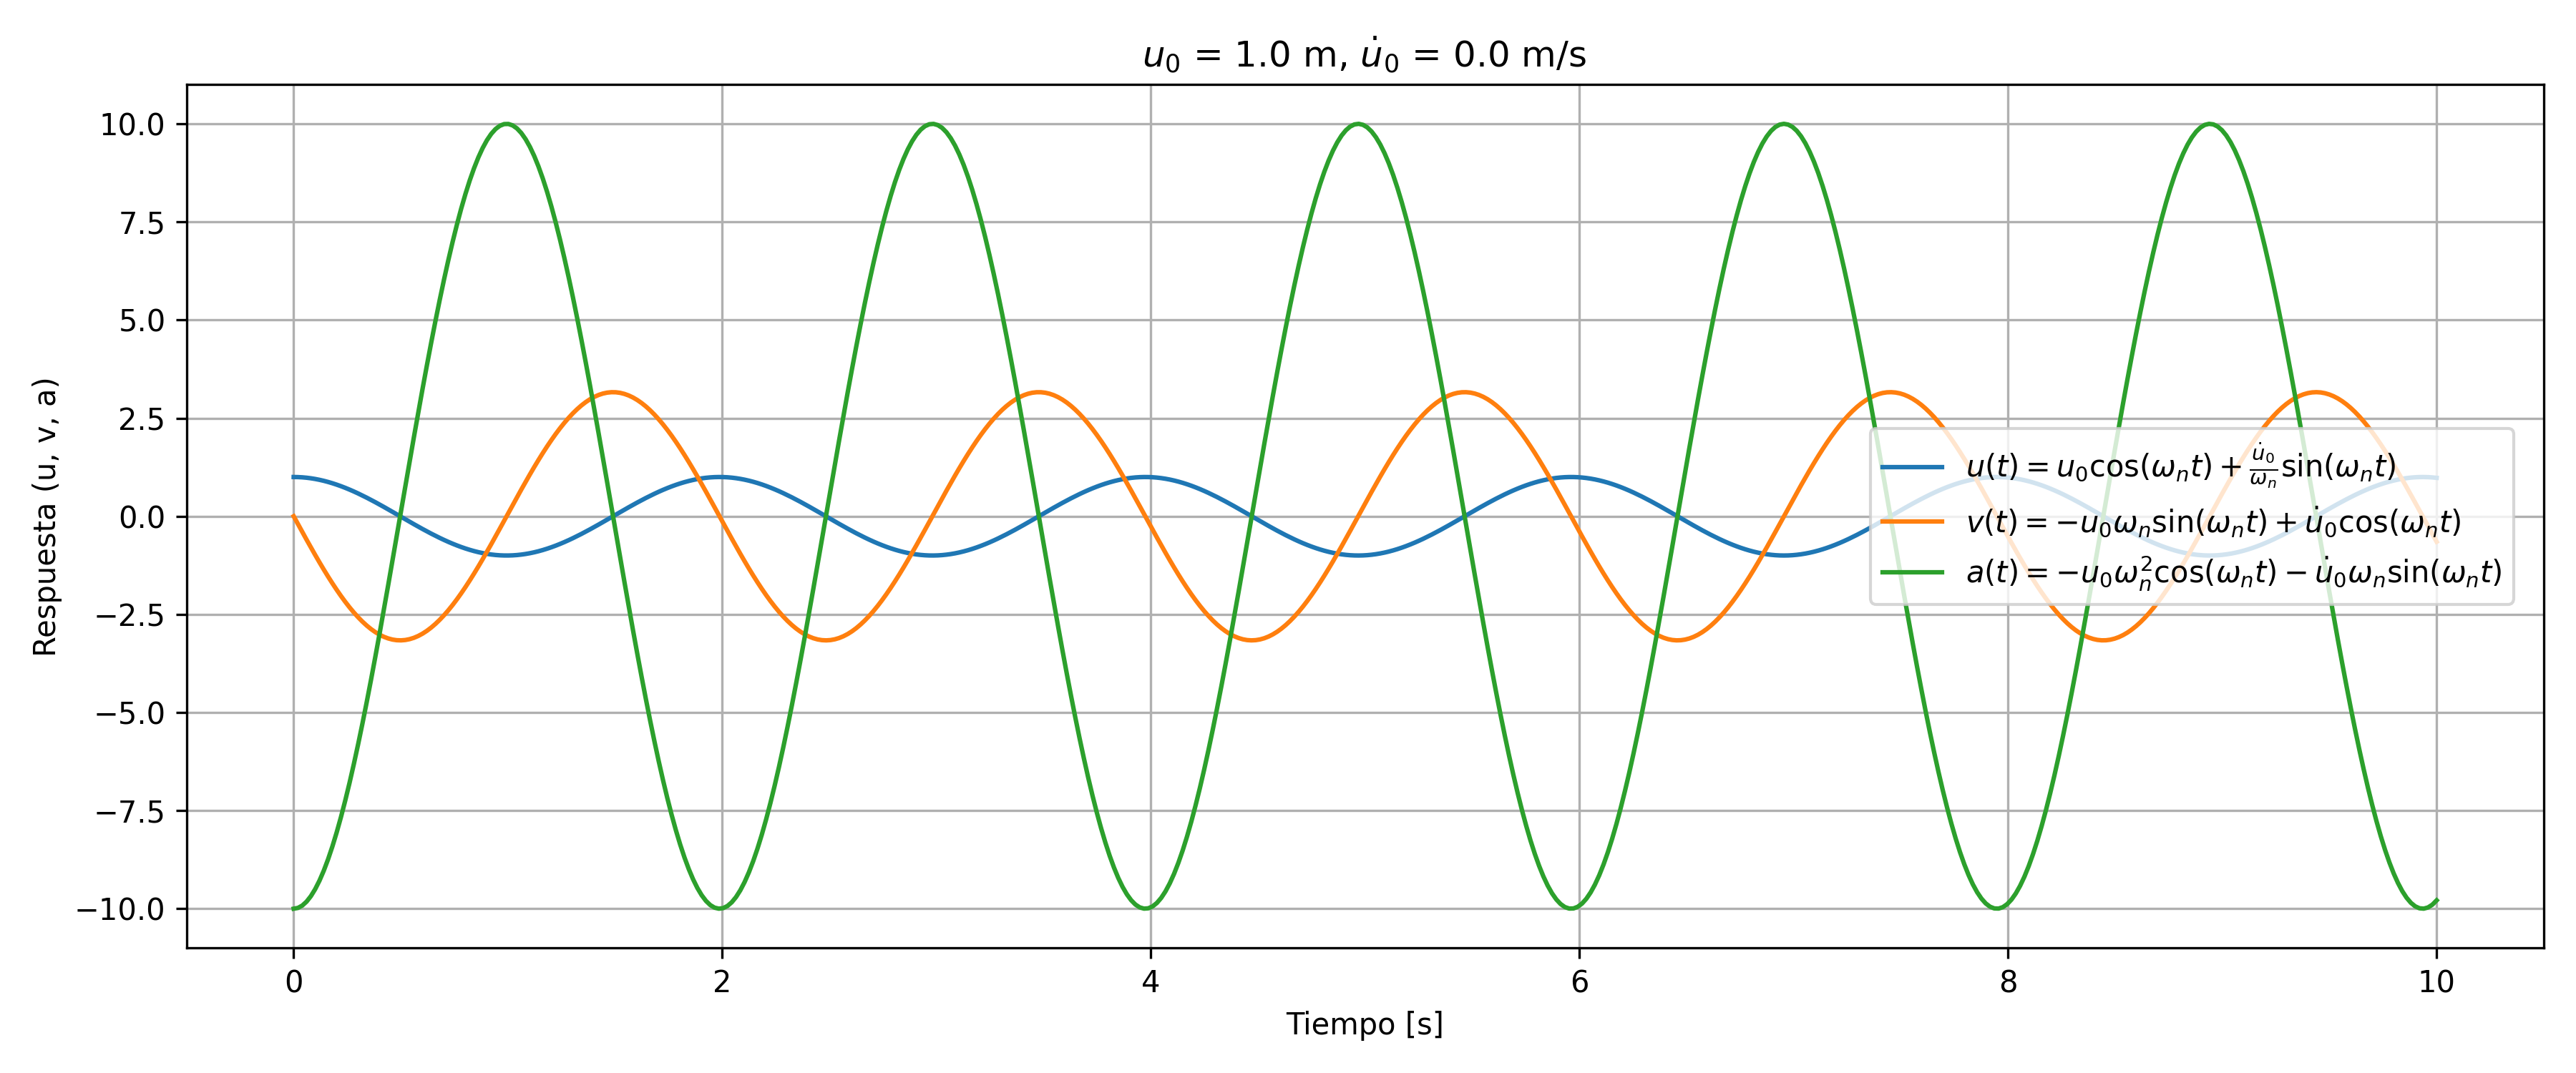
\includegraphics[width=0.8\textwidth]{GRAFICOS/sis_no_amortiguado_u0_1.0_v0_0.0.png}
    \caption{Desplazamiento inicial 1.0, velocidad inicial 0.0}
    \label{fig:ejemplo1}
\end{figure}

\begin{figure}[H]
    \centering
    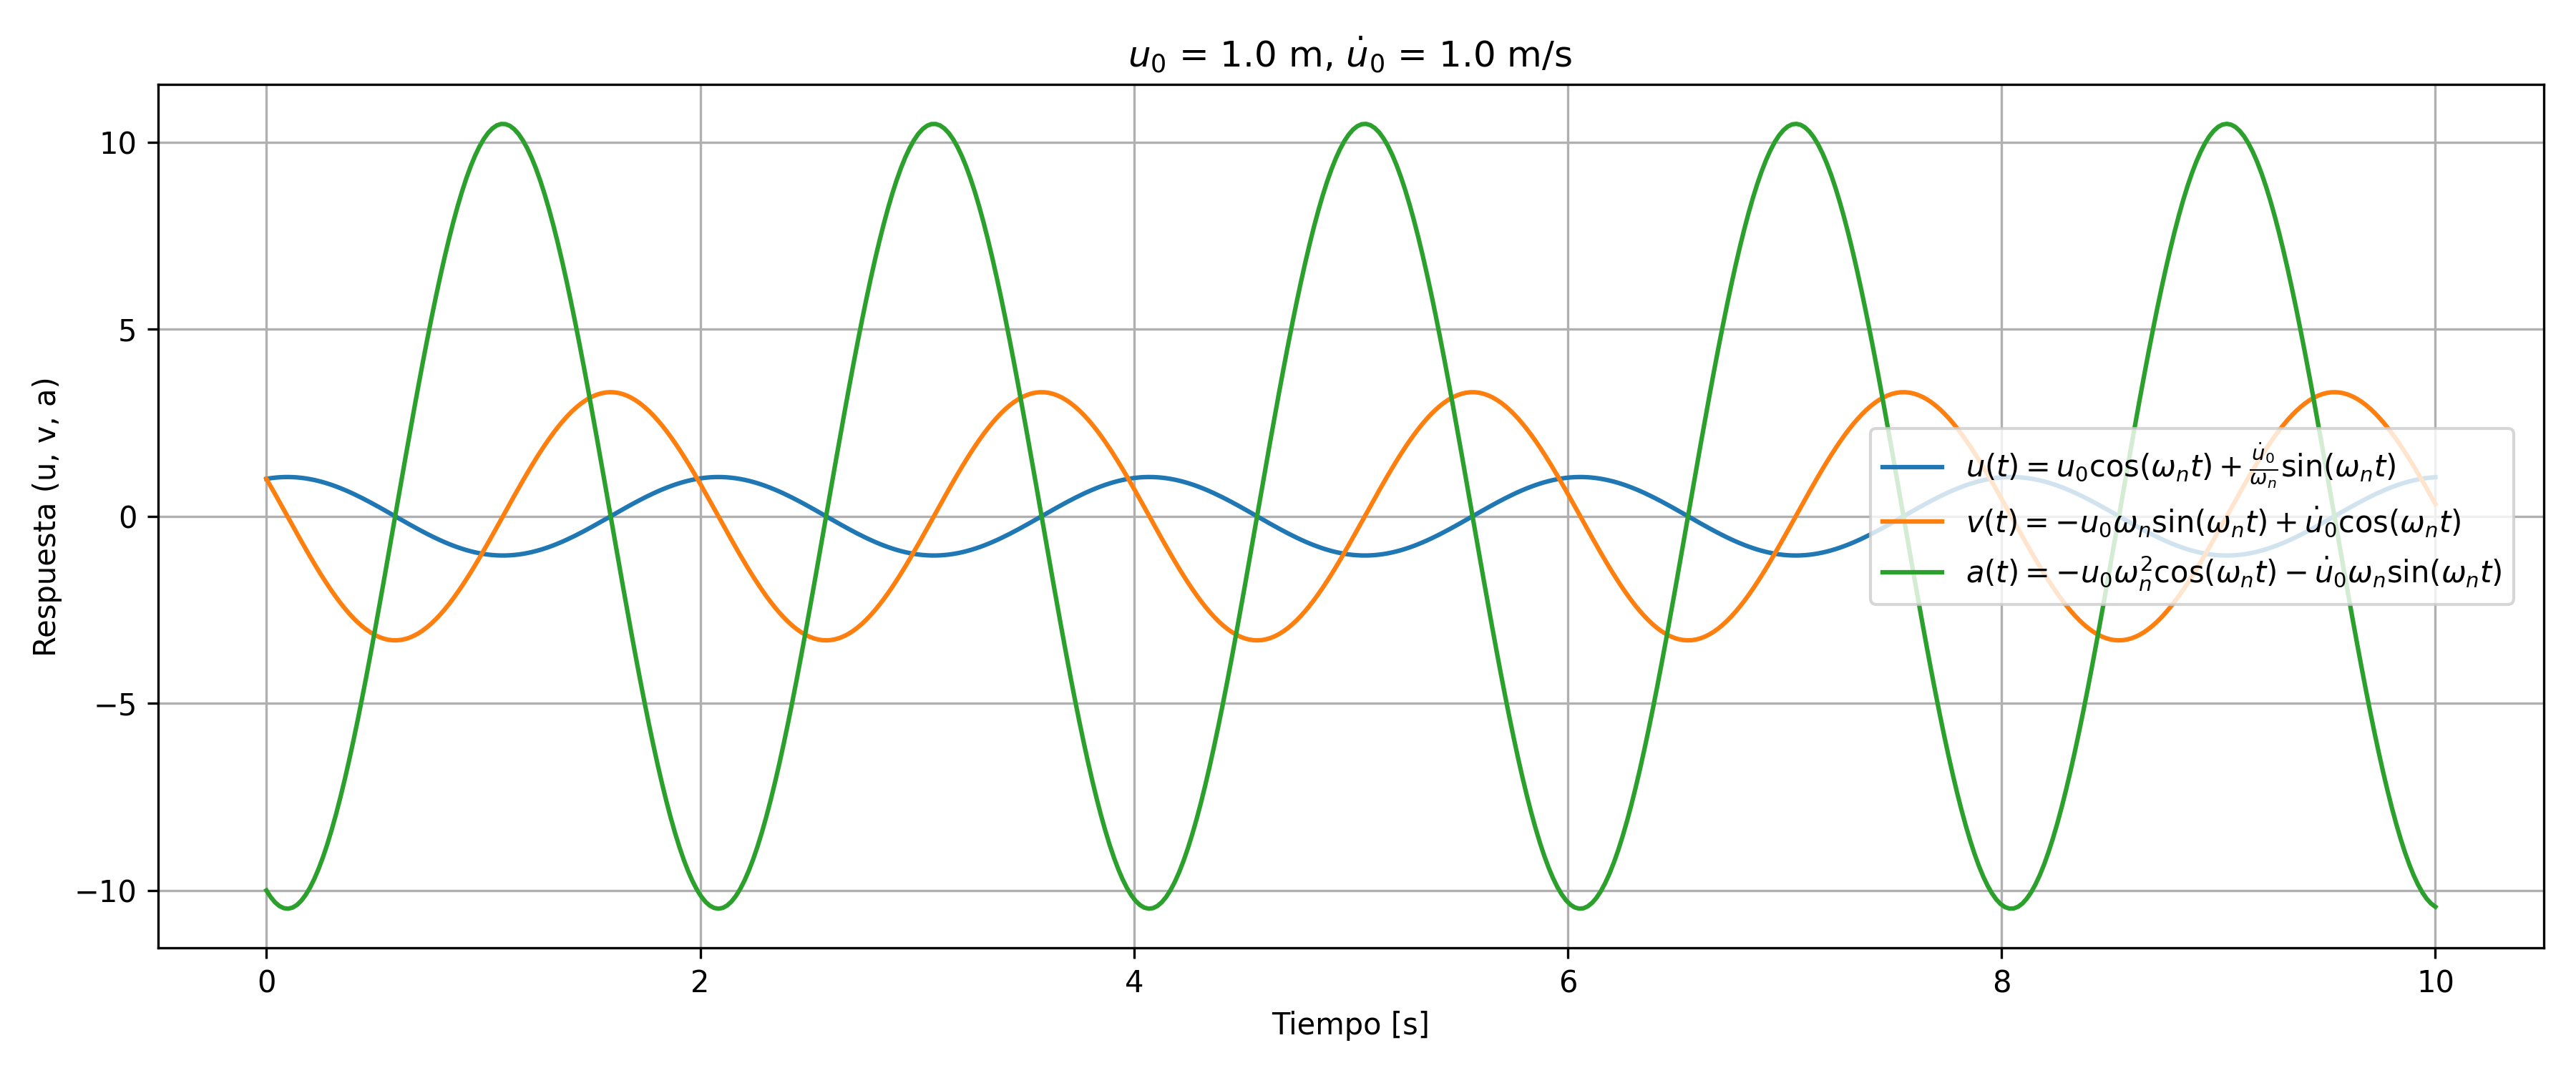
\includegraphics[width=0.8\textwidth]{GRAFICOS/sis_no_amortiguado_u0_1.0_v0_1.0.png}
    \caption{Desplazamiento inicial 1.0, velocidad inicial 1.0}
    \label{fig:ejemplo1}
\end{figure}


\newpage
\section{Vibraciones Libres Armortiguadas}

Se define la ecuacion de movimiento como:
\begin{equation}
    m \ddot{x} + c \dot{x} + kx = 0
\end{equation}

La solucion de la ecuacion del caso homogeneo se supone como:

\begin{equation}
    u(t) = e^{St}
\end{equation}

Derivando, se obtiene la velocidad y aceleracion como:

\begin{equation}
    \dot{u}(t) = Se^{St} \quad \text{y} \quad \ddot{u}(t) = S^2 e^{St}
\end{equation}

Luego, la solucion de la ecuacion para p(t) = 0 es:

\begin{equation}
    S_{1,2} =  \frac{-c}{2m} \pm \omega_n \sqrt{(\frac{c}{2m\omega_n})^2 - 1}
\end{equation}

Luego existen 3 tipos de sistemas:
\begin{itemize}
    \item \textbf{Sobreamortiguado:} $(\frac{c}{2m\omega_n})^2 > 1 \rightarrow S_{1,2} \in \mathbb{R}$ 
    \item \textbf{Criticamente amortiguado:} $(\frac{c}{2m\omega_n})^2 = 1  \rightarrow S_{1,2} = \frac{-c}{2m}$
    \item \textbf{Subamortiguado:} $(\frac{c}{2m\omega_n})^2 < 1 \rightarrow S_{1,2} \in \mathbb{C}$
\end{itemize}

Se define la razon de amortiguamiento critico como:

\begin{equation}
    \beta = \zeta = \frac{c}{c_c} = \frac{c}{2m\omega_n}
\end{equation}

Por lo tanto, la razon de armortiguamiento para los distintos casos es:

\begin{itemize}
    \item \textbf{Sobreamortiguado:} $\beta > 1$
    \item \textbf{Criticamente amortiguado:} $\beta = 1$
    \item \textbf{Subamortiguado:} $\beta < 1$
\end{itemize}

Ademas, se define la frecuencia amortiguada como:

\begin{equation}
    \omega_d = \omega_n \sqrt{\beta^2 - 1} \quad \text{para} \quad \beta >= 1
\end{equation}

\begin{equation}
    \omega_d = \omega_n \sqrt{1 - \beta^2} \quad \text{para} \quad \beta < 1
\end{equation}
\subsection{Sobreamortiguado}

La ecuacion de movimiento se puede escribir como:

\begin{equation}
    u(t) = G_1 e^{-(\beta \omega_n t + \omega_d)t} + G_2 e^{-(\beta \omega_n t - \omega_d)t} \quad G_1, G_2 \in \mathbb{R}
\end{equation}

Lo cual puedo trabajar como:

\begin{equation}
    u_h(t) = e^{-\beta \omega_n t} (G_1 e^{\omega_d t} + G_2 e^{-\omega_d t}) 
\end{equation}

\begin{equation}
    \dot{u}_h(t) = -\beta \omega_n e^{-\beta \omega_n t} (G_1 e^{\omega_d t} + G_2 e^{-\omega_d t}) + e^{-\beta \omega_n t} (G_1 \omega_d e^{\omega_d t} - G_2 \omega_d e^{-\omega_d t})
\end{equation}

\begin{equation}
    \ddot{u}_h(t) = \beta^2 \omega_n^2 e^{-\beta \omega_n t} (G_1 e^{\omega_d t} + G_2 e^{-\omega_d t}) - 2\beta \omega_n e^{-\beta \omega_n t} (G_1 \omega_d e^{\omega_d t} - G_2 \omega_d e^{-\omega_d t}) + e^{-\beta \omega_n t} (G_1 \omega_d^2 e^{\omega_d t} + G_2 \omega_d^2 e^{-\omega_d t})
\end{equation}

Luego para graficar hay que considerar las funciones hiperbólicas, donde:

\begin{equation}
    \sinh(\alpha) = \frac{e^{\alpha} - e^{-\alpha}}{2} \quad \text{y} \quad \cosh(\alpha) = \frac{e^{\alpha} + e^{-\alpha}}{2}
\end{equation}

Algunos ejemplos son:

\begin{figure}[H]
    \centering
    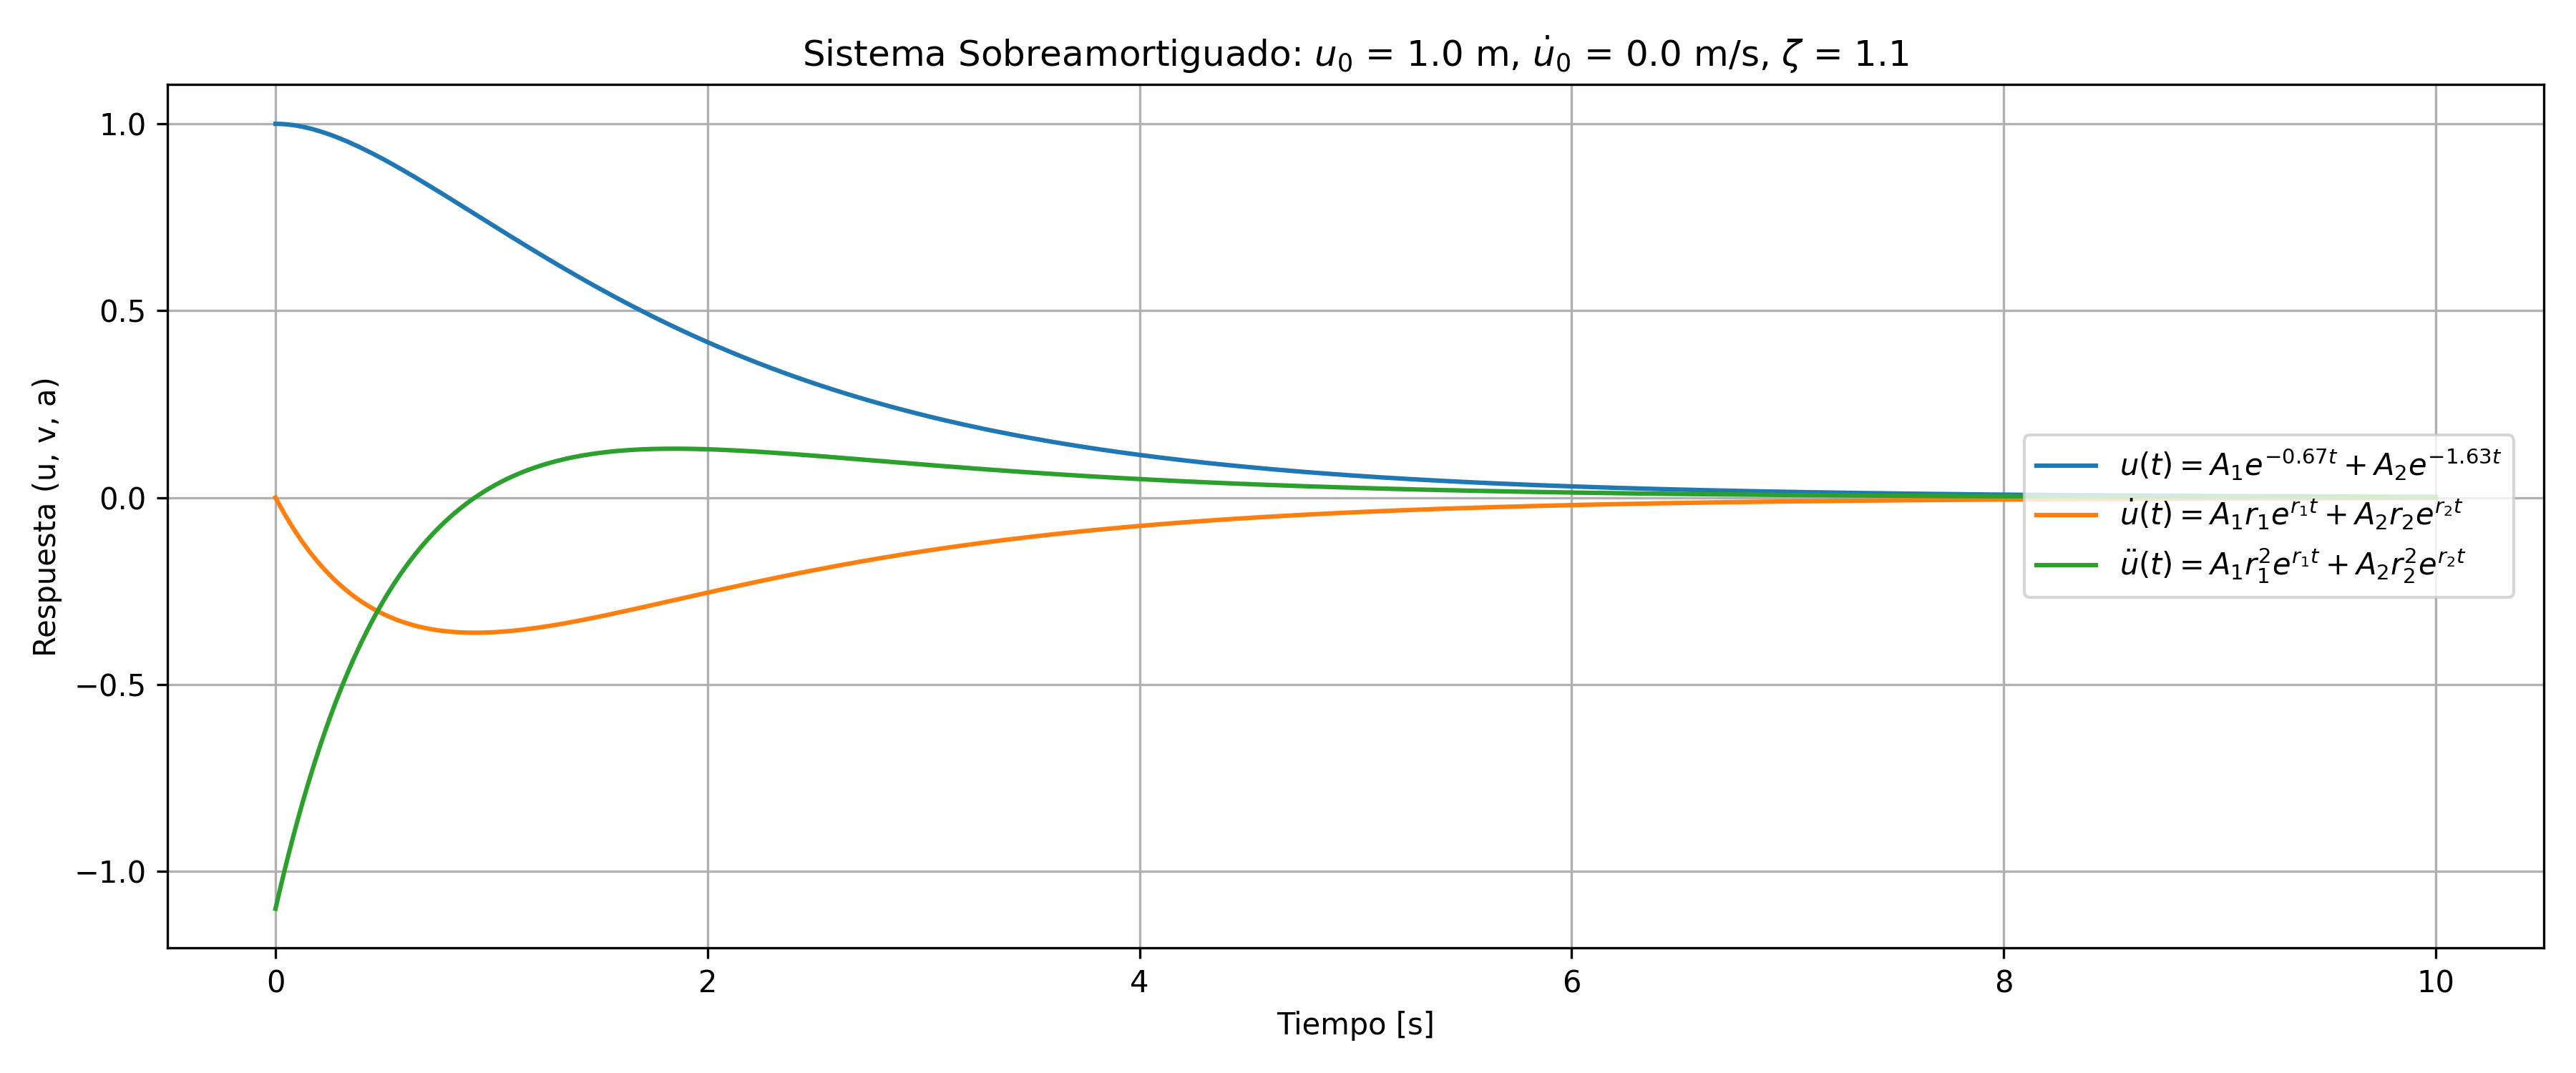
\includegraphics[width=0.8\textwidth]{GRAFICOS/sis_sobreamortiguado_u0_1.0_v0_0.0_zeta_1.1.png}
    \caption{Desplazamiento inicial 1.0, velocidad inicial 0.0}
    \label{fig:ejemplo1}
\end{figure}

\begin{figure}[H]
    \centering
    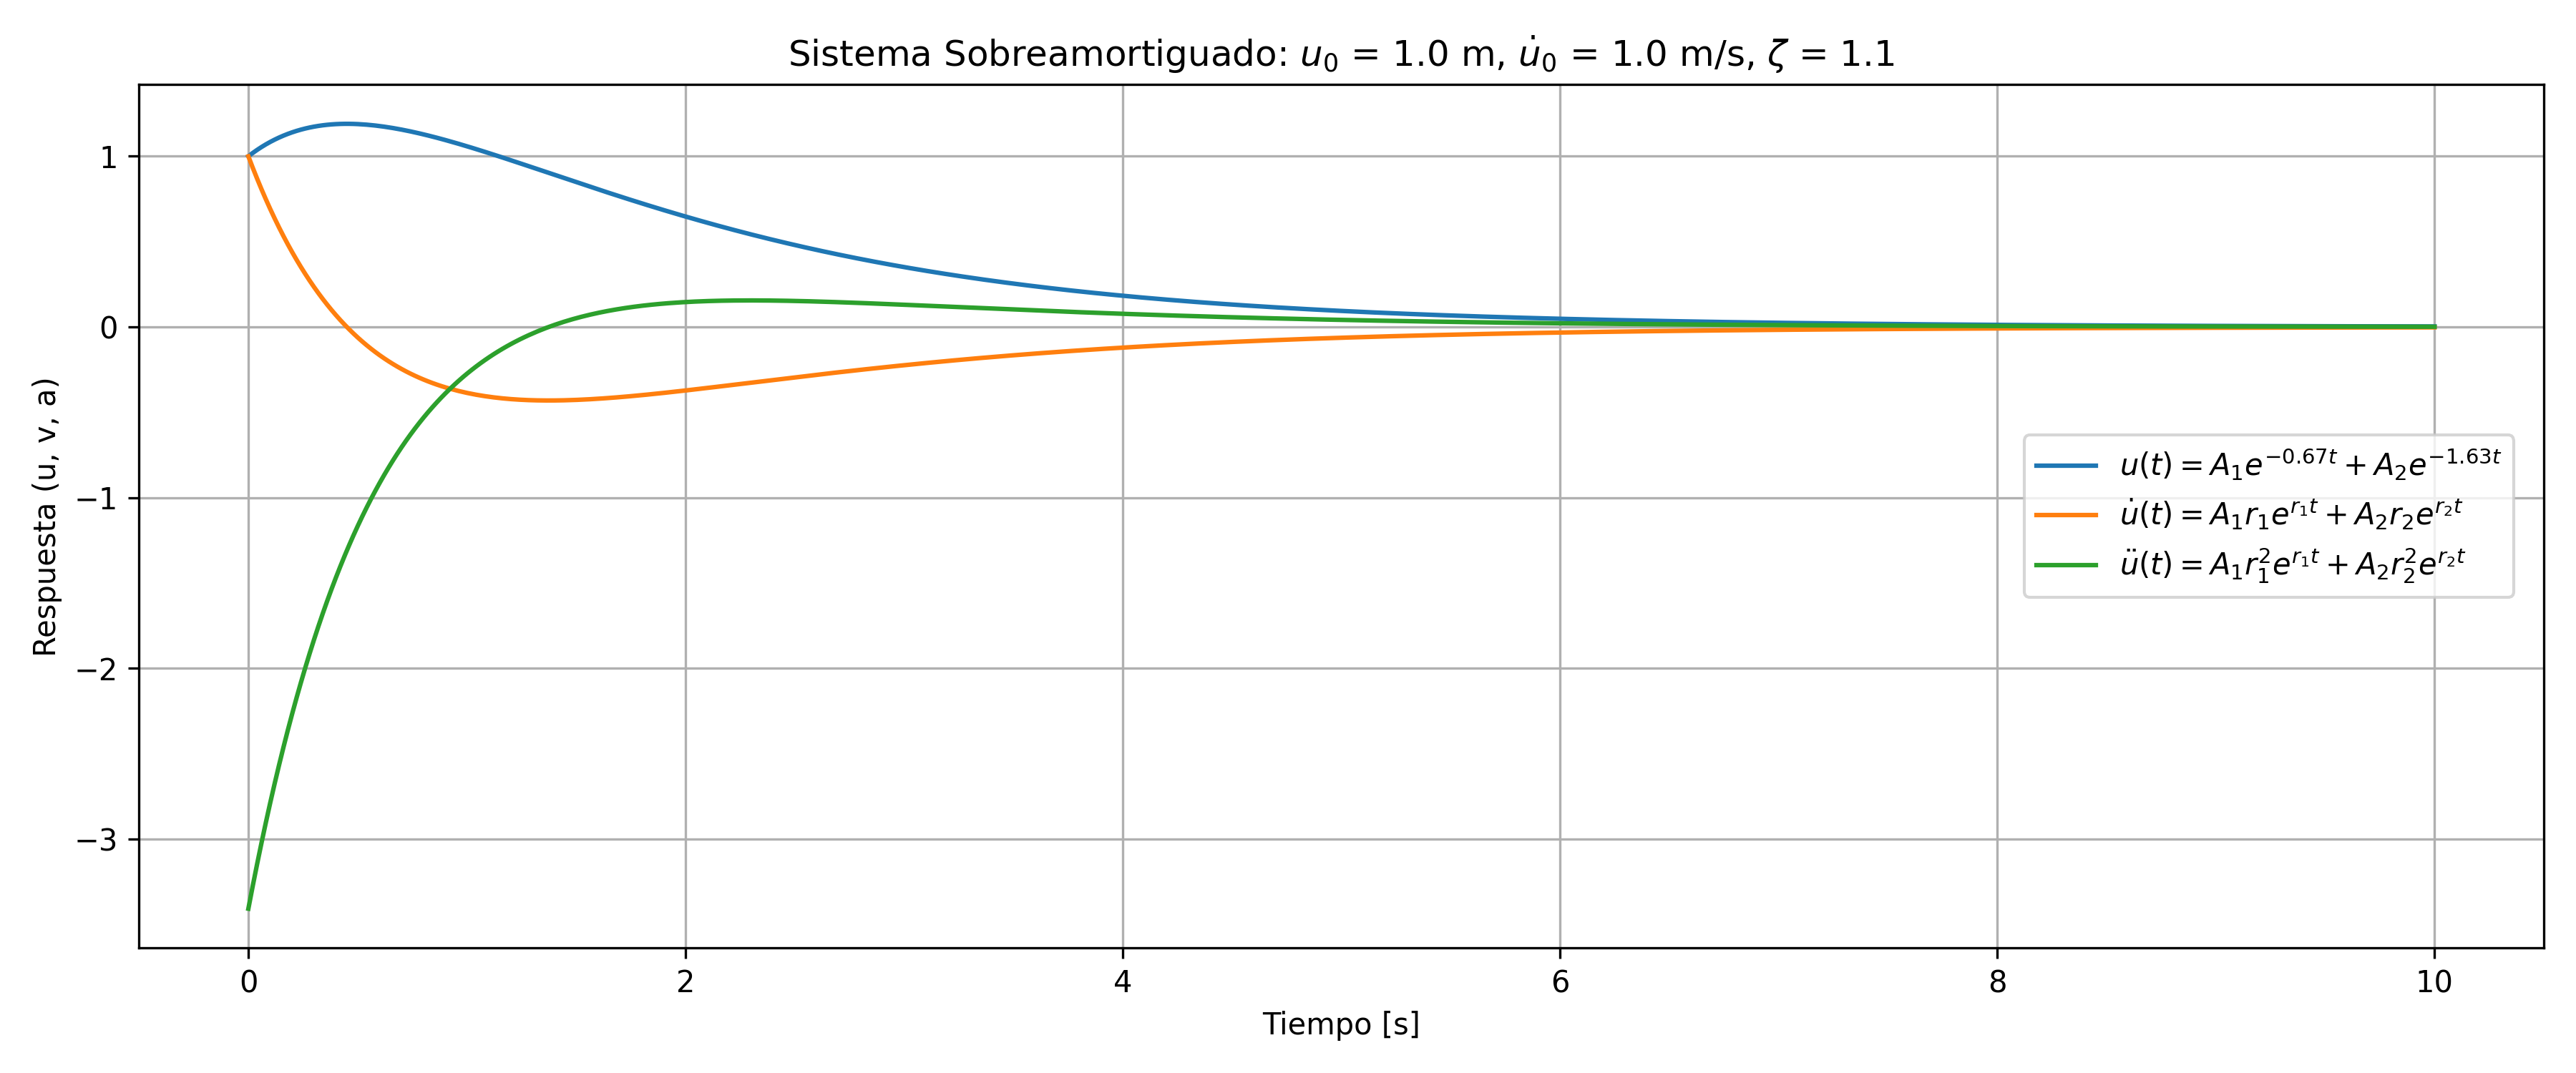
\includegraphics[width=0.8\textwidth]{GRAFICOS/sis_sobreamortiguado_u0_1.0_v0_1.0_zeta_1.1.png}
    \caption{Desplazamiento inicial 1.0, velocidad inicial 1.0}
    \label{fig:ejemplo1}
\end{figure}

\subsection{Criticamente amortiguado}

Las soluciones a la ecuacion de movimiento son:

\begin{equation}
   S_{1,2} = -\beta \omega_n = \omega_n
\end{equation}

Por lo tanto:

\begin{equation}
    u(t) = G_1e^{-\omega_n t} 
\end{equation}
\begin{equation}
    u_2(t) = G_2e^{-\omega_n t}
\end{equation}

Luego:

\begin{equation}
    u_h(t) = G_1e^{-\omega_n t} + G_2te^{-\omega_n t} \quad G_1, G_2 \in \mathbb{R}
\end{equation}

\begin{equation}
    \dot{u}_h(t) = -\omega_n G_1e^{-\omega_n t} + G_2e^{-\omega_n t} - G_2\omega_n te^{-\omega_n t}
\end{equation}

\begin{equation}
    \ddot{u}_h(t) = \omega_n^2 G_1e^{-\omega_n t} - 2\omega_n G_2e^{-\omega_n t} + G_2\omega_n^2 te^{-\omega_n t}
\end{equation}

Algunos ejemplos son:
\begin{figure}[H]
    \centering
    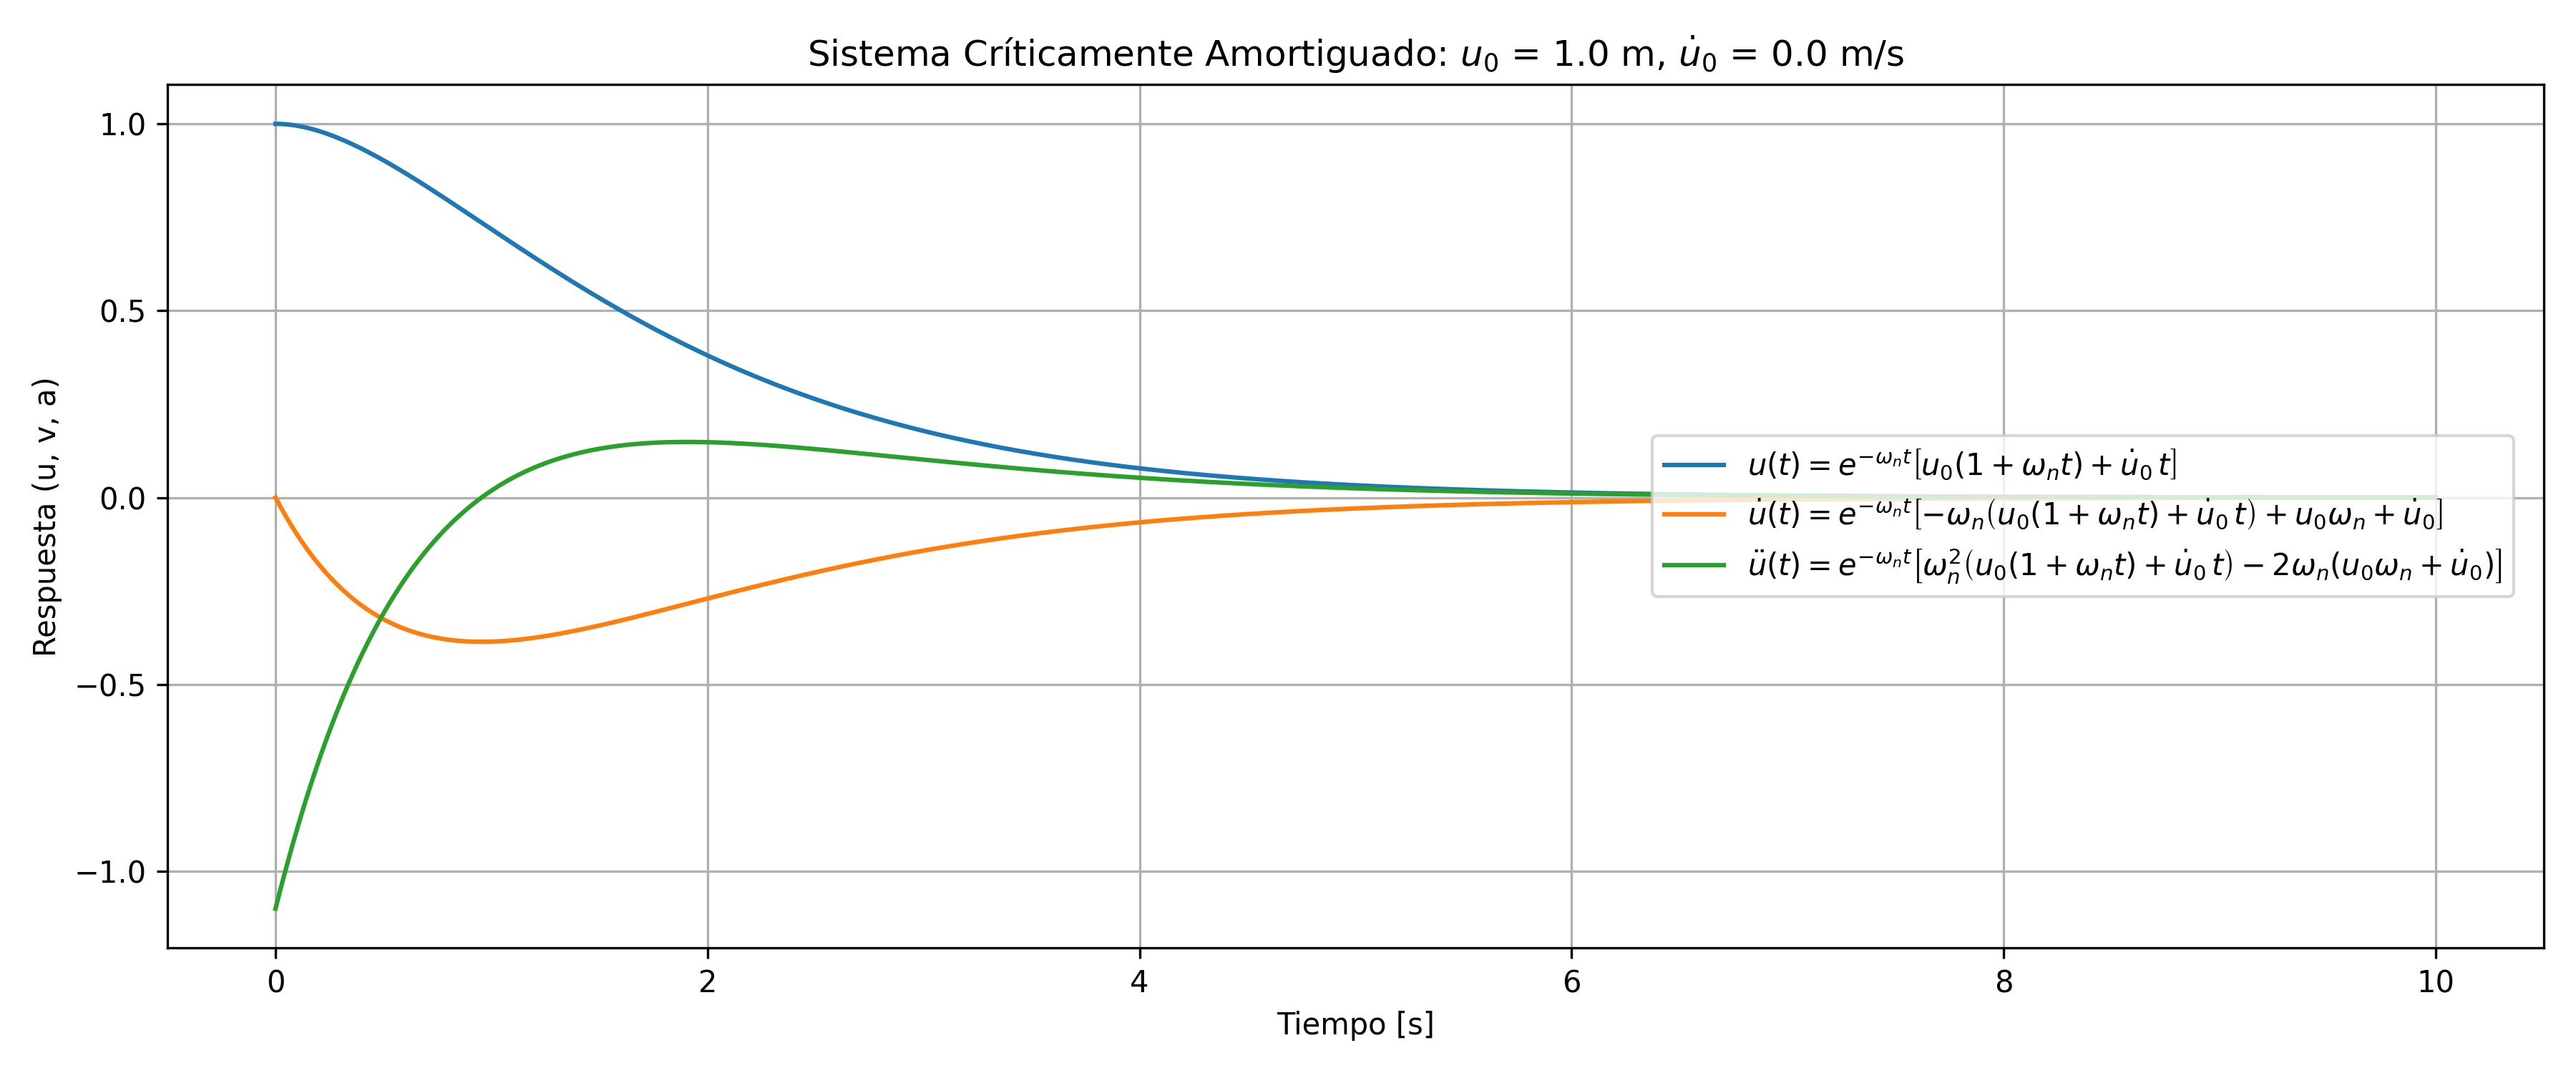
\includegraphics[width=0.8\textwidth]{GRAFICOS/sis_criticamente_amortiguado_u0_1.0_v0_0.0.png}
    \caption{Desplazamiento inicial 1.0, velocidad inicial 0.0}
    \label{fig:ejemplo1}
\end{figure}

\begin{figure}[H]
    \centering
    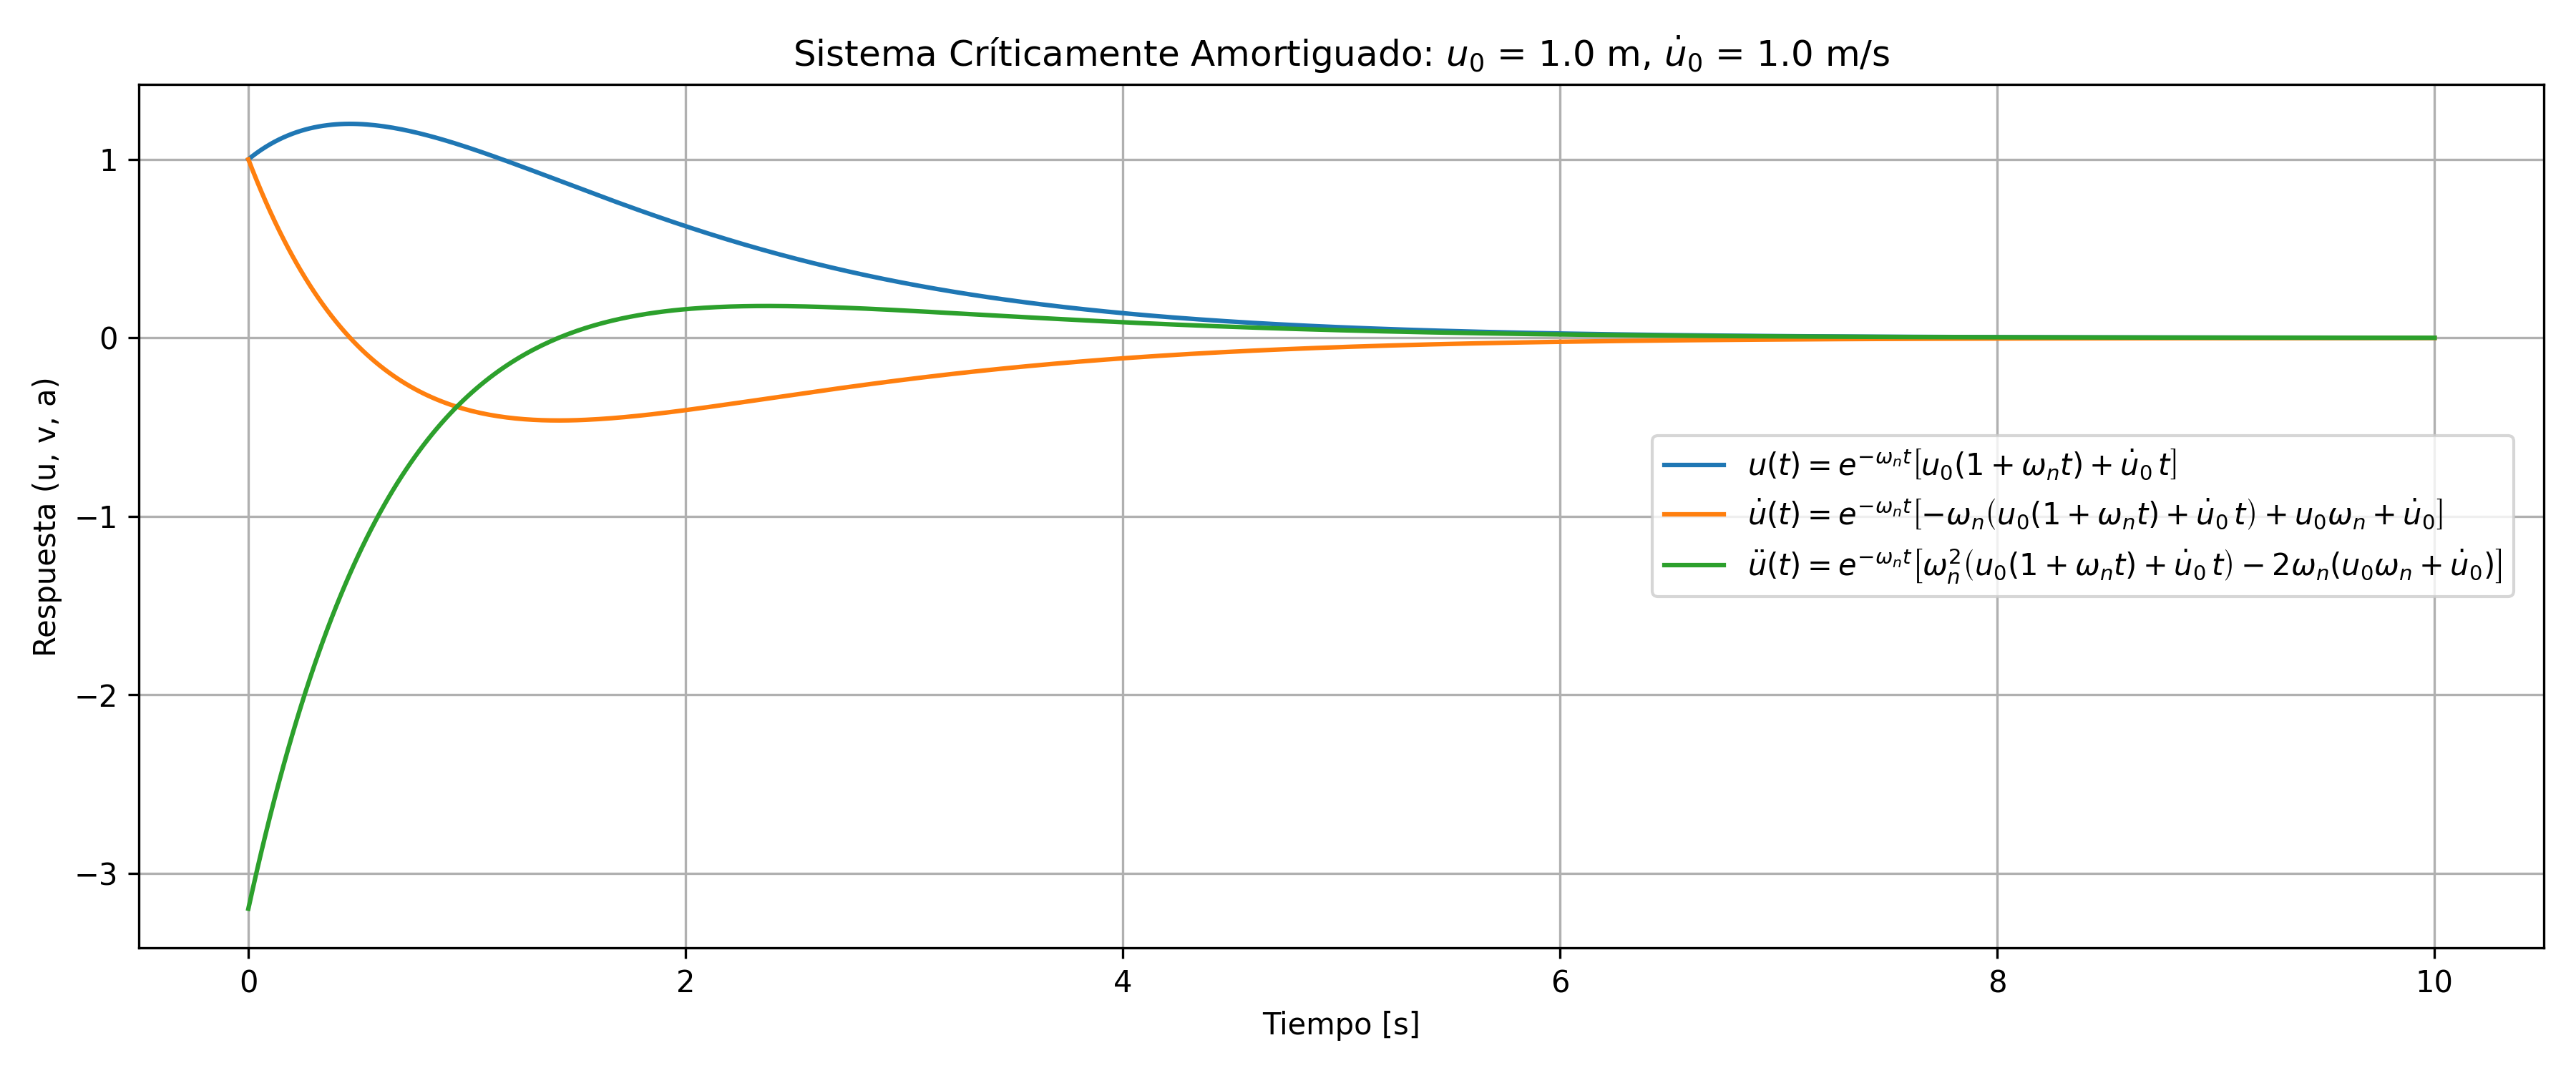
\includegraphics[width=0.8\textwidth]{GRAFICOS/sis_criticamente_amortiguado_u0_1.0_v0_1.0.png}
    \caption{Desplazamiento inicial 1.0, velocidad inicial 1.0}
    \label{fig:ejemplo1}
\end{figure}

\subsection{Subamortiguado}

Recordar que en este caso:

\begin{equation}
    \omega_d = \omega_n \sqrt{1 - \beta^2}
\end{equation}

Luego la ecuacion de movimiento se puede escribir como:

\begin{equation}
    u(t) = G_1 e^{-\beta \omega_n t + j \omega_d t} + G_2 e^{-\beta \omega_n t - j \omega_d t} \quad G_1, G_2 \in \mathbb{C}
\end{equation}

Por lo tanto, se pueden escribir las constantes $G_1$ y $G_2$ como:

\begin{equation}
    G_1 = C_1 + jC_2 \quad G_2 = C_3 + jC_4 \quad C_1, C_2, C_3, C_4 \in \mathbb{R}
\end{equation}

Ademas, se puede escribir $e^{j\alpha}$ como:
\begin{equation}
    e^{j\alpha} = \cos(\alpha) + j\sin(\alpha) \quad \text{y} \quad e^{-j\alpha} = \cos(\alpha) - j\sin(\alpha)
\end{equation}

Por lo tanto, se debe cumplir que:

\begin{equation}
    C_2 + C_4 = 0 \quad \text{y} \quad C_1 - C_3 = 0
\end{equation}

Sea:

\begin{equation}
    A = C4 - C2 \quad \text{y} \quad B = C1 + C3
\end{equation}

Luego la ecuacion de movimiento se puede escribir como:

\begin{equation}
    u_h(t) = e^{-\beta \omega_n t} (A \sin(\omega_d t) + B \cos(\omega_d t)) \quad \beta \in [0, 1[
\end{equation}

\begin{equation}
    \dot{u}_h(t) = -\beta \omega_n e^{-\beta \omega_n t} (A \sin(\omega_d t) + B \cos(\omega_d t)) + e^{-\beta \omega_n t} (A \omega_d \cos(\omega_d t) - B \omega_d \sin(\omega_d t))
\end{equation}

\begin{align}
    \ddot{u}_h(t) &= \beta^2 \omega_n^2 e^{-\beta \omega_n t} (A \sin(\omega_d t) + B \cos(\omega_d t)) \notag \\
    &\quad - 2\beta \omega_n e^{-\beta \omega_n t} (A \omega_d \cos(\omega_d t) - B \omega_d \sin(\omega_d t)) \notag \\
    &\quad + e^{-\beta \omega_n t} (A \omega_d^2 \sin(\omega_d t) + B \omega_d^2 \cos(\omega_d t))
\end{align}
    
Lo cual se puede simplificar como:

\begin{equation}
    u_h(t) = \rho e^{-\beta \omega_n t} \cos(\omega_d t - \phi) \quad \text{donde} \quad \rho = \sqrt{A^2 + B^2} \quad \text{y} \quad \phi = \tan^{-1}(\frac{A}{B})
\end{equation}

\begin{equation}
    \dot{u}_h(t) = -\rho \beta \omega_n e^{-\beta \omega_n t} \cos(\omega_d t - \phi -\phi_1) \quad \text{donde} \quad \phi_1 = \tan^(-1)\frac{\sqrt{1-\beta^2}}{\beta}
\end{equation}

\begin{equation}
    \ddot{u}_h(t) = -\rho \omega_n^2 e^{-\beta \omega_n t} \cos(\omega_d t - \phi - 2\phi_1)
\end{equation}

Algunos ejemplos son:

\begin{figure}[H]
    \centering
    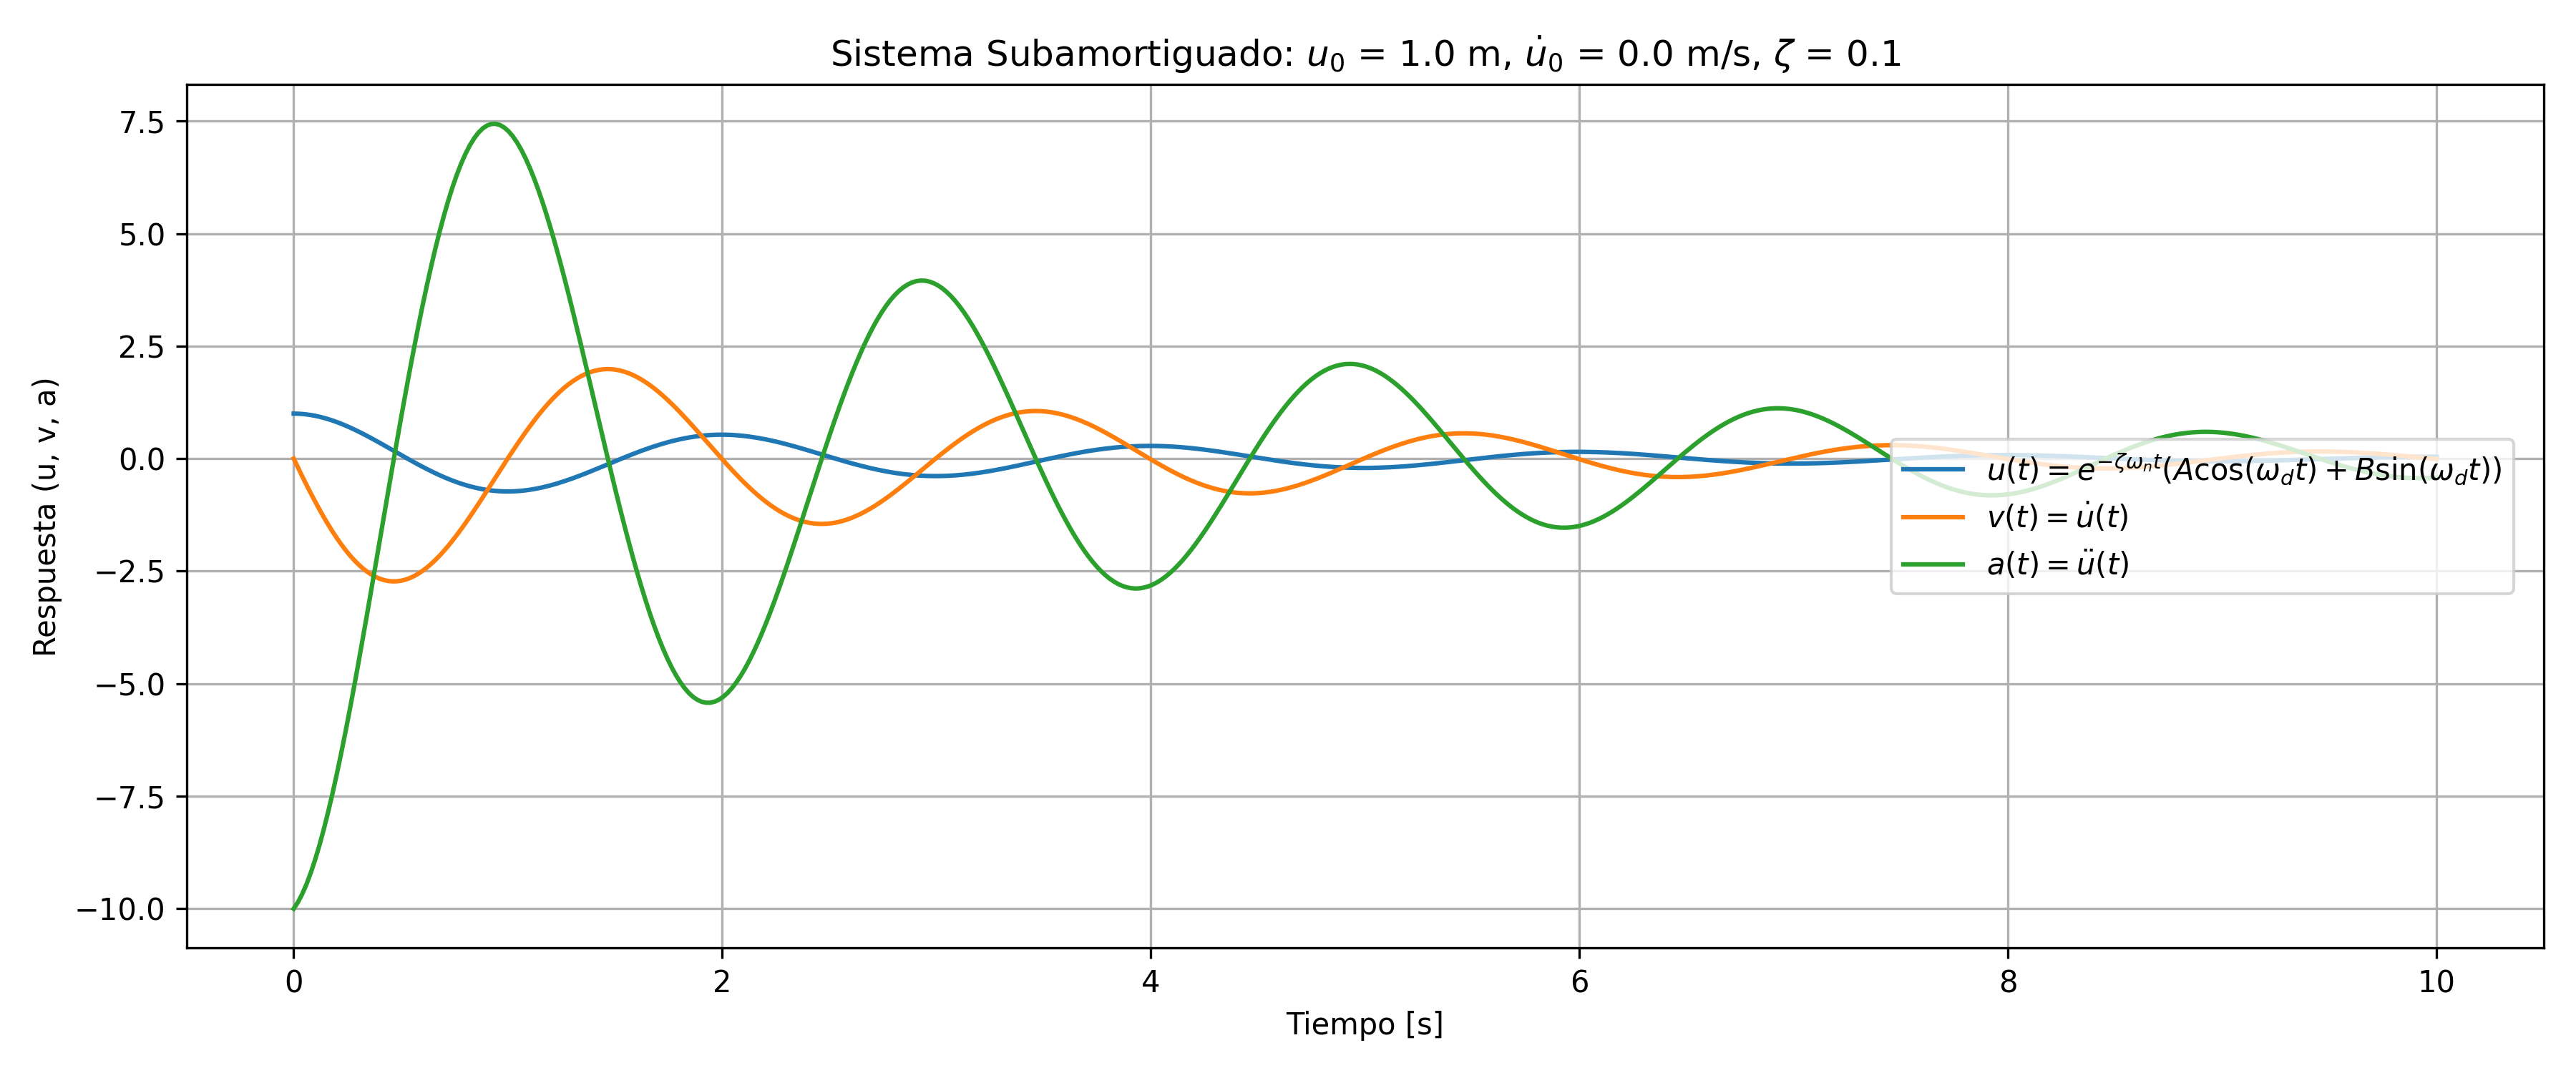
\includegraphics[width=0.8\textwidth]{GRAFICOS/sis_subamortiguado_u0_1.0_v0_0.0_zeta_0.1.png}
    \caption{Desplazamiento inicial 1.0, velocidad inicial 0.0}
    \label{fig:ejemplo1}
\end{figure}

\begin{figure}[H]
    \centering
    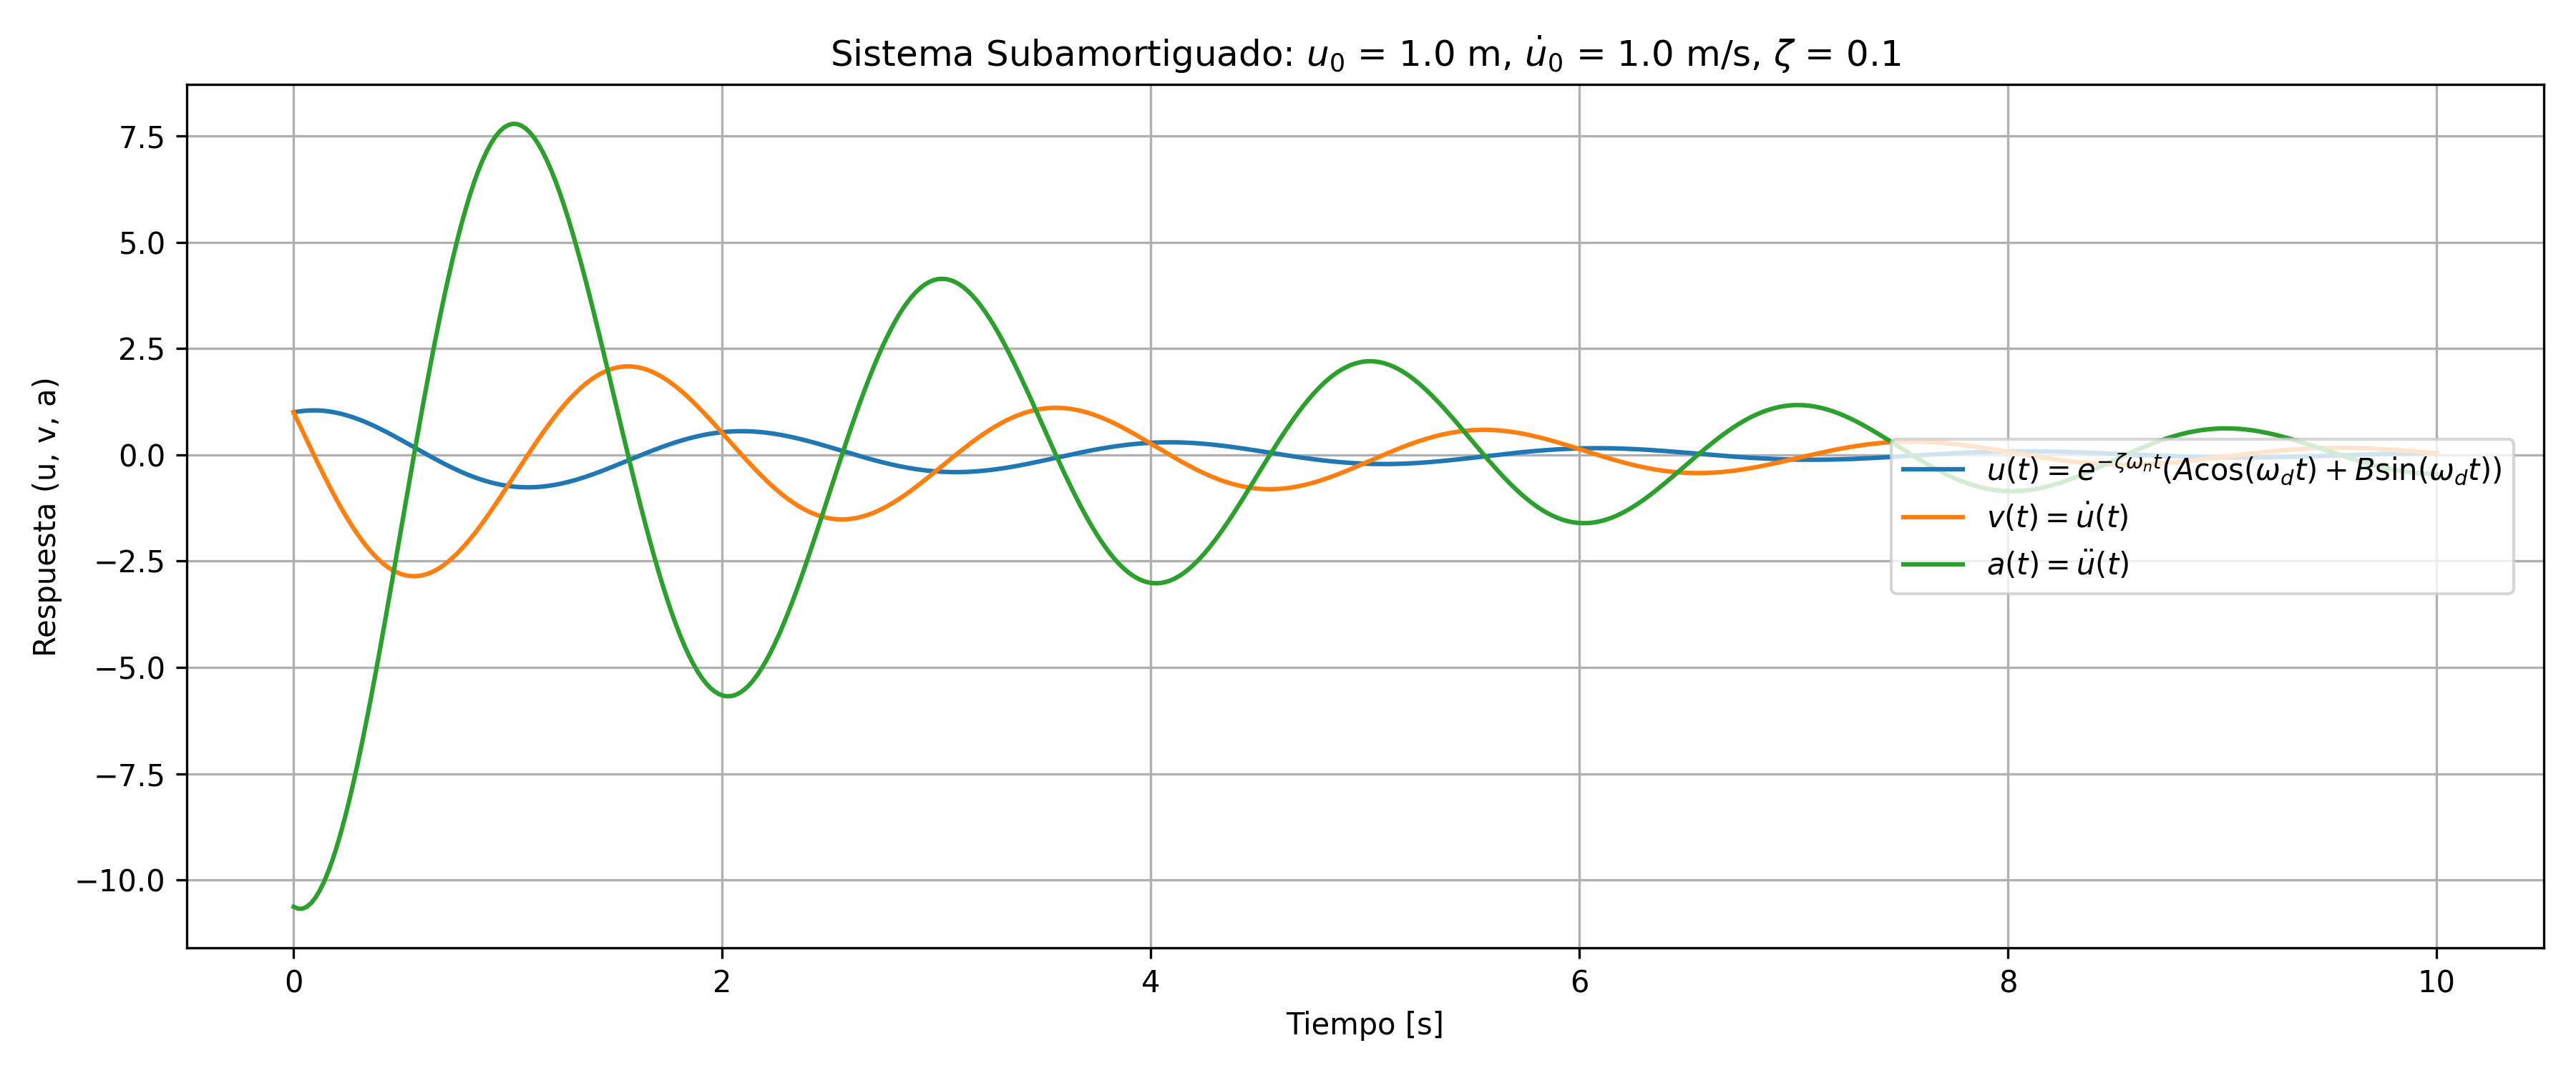
\includegraphics[width=0.8\textwidth]{GRAFICOS/sis_subamortiguado_u0_1.0_v0_1.0_zeta_0.1.png}
    \caption{Desplazamiento inicial 1.0, velocidad inicial 1.0}
    \label{fig:ejemplo1}
\end{figure}

\section{Interpolacion a partir de mediciones}

Si se generan mediciones de estudio, se puede generar una interpolacion a partir de estas, por ejemplo:

\begin{table}[H]
    \centering
    \begin{tabular}{p{3.5cm} >{\centering\arraybackslash}p{2.5cm} >{\centering\arraybackslash}p{2.5cm}}
        \toprule
        \textbf{Amp (cm)} & \textbf{Tiempo (s)}  \\
        \midrule
        6.0  & 0.4\\
        -4.66  & 1.0\\
        3.62  & 1.6\\
        -2.82  & 2.21\\
        2.19  & 2.81\\
        -1.7  & 3.41\\
        1.32  & 4.01\\
        -1.18  & 4.61\\
        1.06  & 5.22\\
        -0.92  & 5.82\\
        0.79  & 6.42\\
        -0.66  & 7.02\\
        0.52  & 7.62\\
        -0.36 & 8.23\\
        \bottomrule
    \end{tabular}
    \caption{Medicion ejemplo.}
    \label{tab:cargas_maximas}
  \end{table}

Luego es posible generar una interpolacion a partir de estas mediciones, por ejemplo:

\begin{figure}[H]
    \centering
    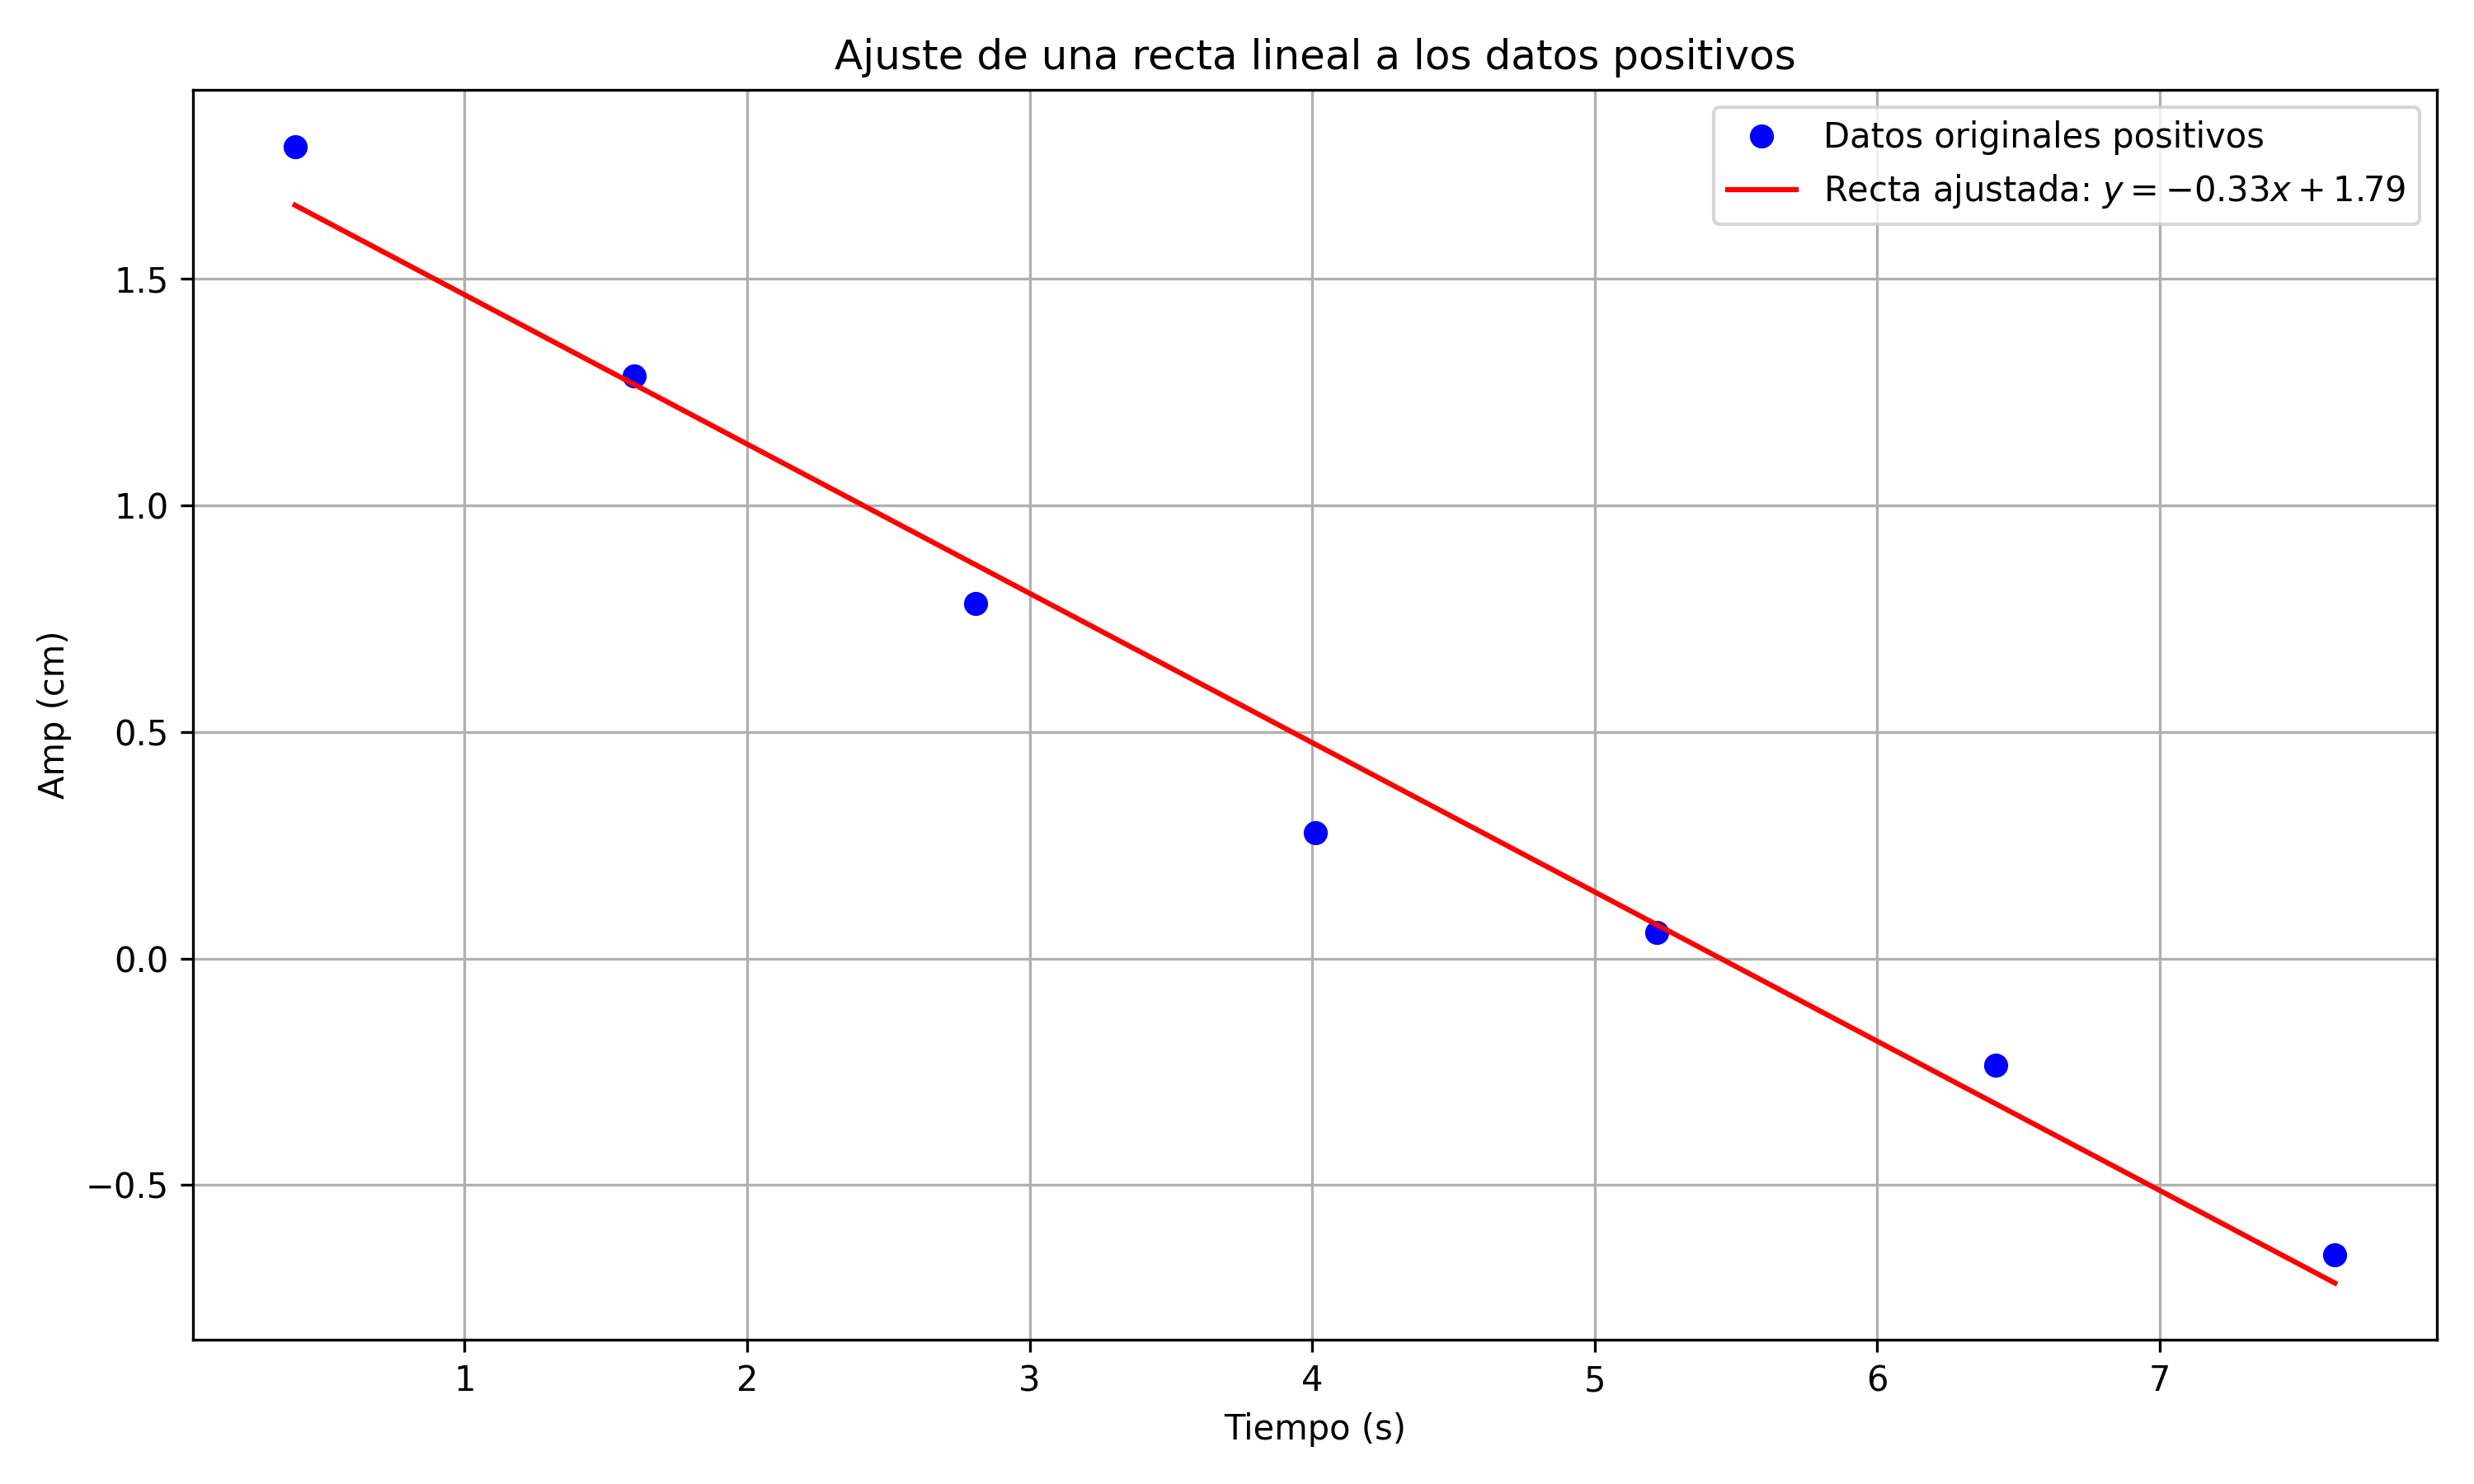
\includegraphics[width=0.6\textwidth]{GRAFICOS/ajuste_recta.png}
    \caption{Interpolacion a partir de mediciones.}
    \label{fig:ejemplo1}
\end{figure}

\textbf{OJO, la implitud debe ir en logaritmo natural}

Luego la recta se puede escribir como:

\begin{equation}
    y = mx + b \quad \text{Analogo a} \quad \ln(u_{max}) = \ln(\rho) - \beta \omega_n t
\end{equation}

Ademas, es posible obtener el periodo armortiguado, asi como la frecuencia armoritugada promediando los intervalos:

\begin{equation}
    T_d = \frac{T_1 + T_2 + T_3 \dots T_n}{N} \quad \text{y} \quad f_d = \frac{1}{T_d}
\end{equation}

Luego sea $b = -\beta \omega_n$, se pueden hacer las siguientes definiciones:

\begin{equation}
    \omega_n = \sqrt{(\frac{2 \pi}{T_d})^2 + b^2 } 
\end{equation}

\section{Cargas Armonicas}

Manteniendo el sistema de un DOF sin armortiguamiento, se puede definir la ecuacion de movimiento como:

\begin{equation}
    m \ddot{x} + c \dot{x} + kx = p_0 \sin(\frac{2\pi}{T_d}t)
\end{equation}

Por lo tanto, la ecuacion homogenes se mantiene:

\begin{equation}
    u_h(t) = A \sin(\omega_n t) + B \cos(\omega_n t)
\end{equation}

Luego, para la solucion particular, se puede escribir como:

\begin{equation}
    u_p(t) = u_p \sin(\bar{\omega} t )
\end{equation}

\begin{equation}
    \dot{u}_p(t) = \bar{\omega} u_p \cos(\bar{\omega} t )
\end{equation}

\begin{equation}
    \ddot{u}_p(t) = -\bar{\omega}^2 u_p \sin(\bar{\omega} t )
\end{equation}

Donde $\bar{\omega}$ corresponde a la frecuencia de la carga armonica. Se puede reescribir la ecuacion de movimiento como:

\begin{equation}
    (-m \bar{\omega}^2 + k)u_p \sin(\bar{\omega} t ) = p_0 \sin(\bar{\omega} t )
\end{equation}

Por lo tanto, $u_p$ equivale a:

\begin{equation}
    u_p = \frac{p_0}{k} \cdot \frac{1}{1-(\frac{\bar{\omega}}{\omega_n})^2}
\end{equation}

Luego:

\begin{equation}
    u_p(t) = \frac{p_0}{k} \cdot \frac{1}{1-(\frac{\bar{\omega}}{\omega_n})^2} \sin{\bar{\omega} t }
\end{equation}

De esta forma, se puede definir $u(t)$ como:

\begin{equation}
    u(t) = \frac{p_0}{k} \cdot \frac{1}{1-(\frac{\bar{\omega}}{\omega_n})^2} \sin{\bar{\omega} t } + A \sin(\omega_n t) + B \cos(\omega_n t)
\end{equation}

Recordando que $\omega_n^2 = \frac{k}{m}$, podemos reescribir $u(t)$ como:

\begin{equation}
    u(t) = \frac{p_0}{k} \cdot \text{FAD}(\frac{\bar\omega}{\omega_n})
\end{equation}

Donde FAD corresponde al Factor de Amplificacion Dinamico, el cual se define como:

\begin{equation}
    \text{FAD}(\frac{\bar\omega}{\omega_n}) = \frac{1}{1-(\frac{\bar{\omega}}{\omega_n})^2}
\end{equation}

Es posible generar una relacion entre la frecuencia de exitacion y la frecuencia natural del sistema:

\begin{equation}
    \lambda = \frac{\bar{\omega}}{\omega_n} = \frac{\bar{f}}{f_n} = \frac{\bar{T}}{T_n}
\end{equation}

De esta forma, $\frac{p_0}{k}$ corresponde a la deformacion estatica, por lo tanto, la respuesta particualr es:

\begin{equation}
    u_p(t) = u_{est} \text{FAD}(\lambda) \sin(\bar{\omega} t)
\end{equation}

Donde FAD de $\lambda$ corresponde a:

\begin{equation}
    \text{FAD}(\lambda) = \frac{1}{1-\lambda^2}
\end{equation}

Lo cual se visualiza como:

\begin{figure}[H]
    \centering
    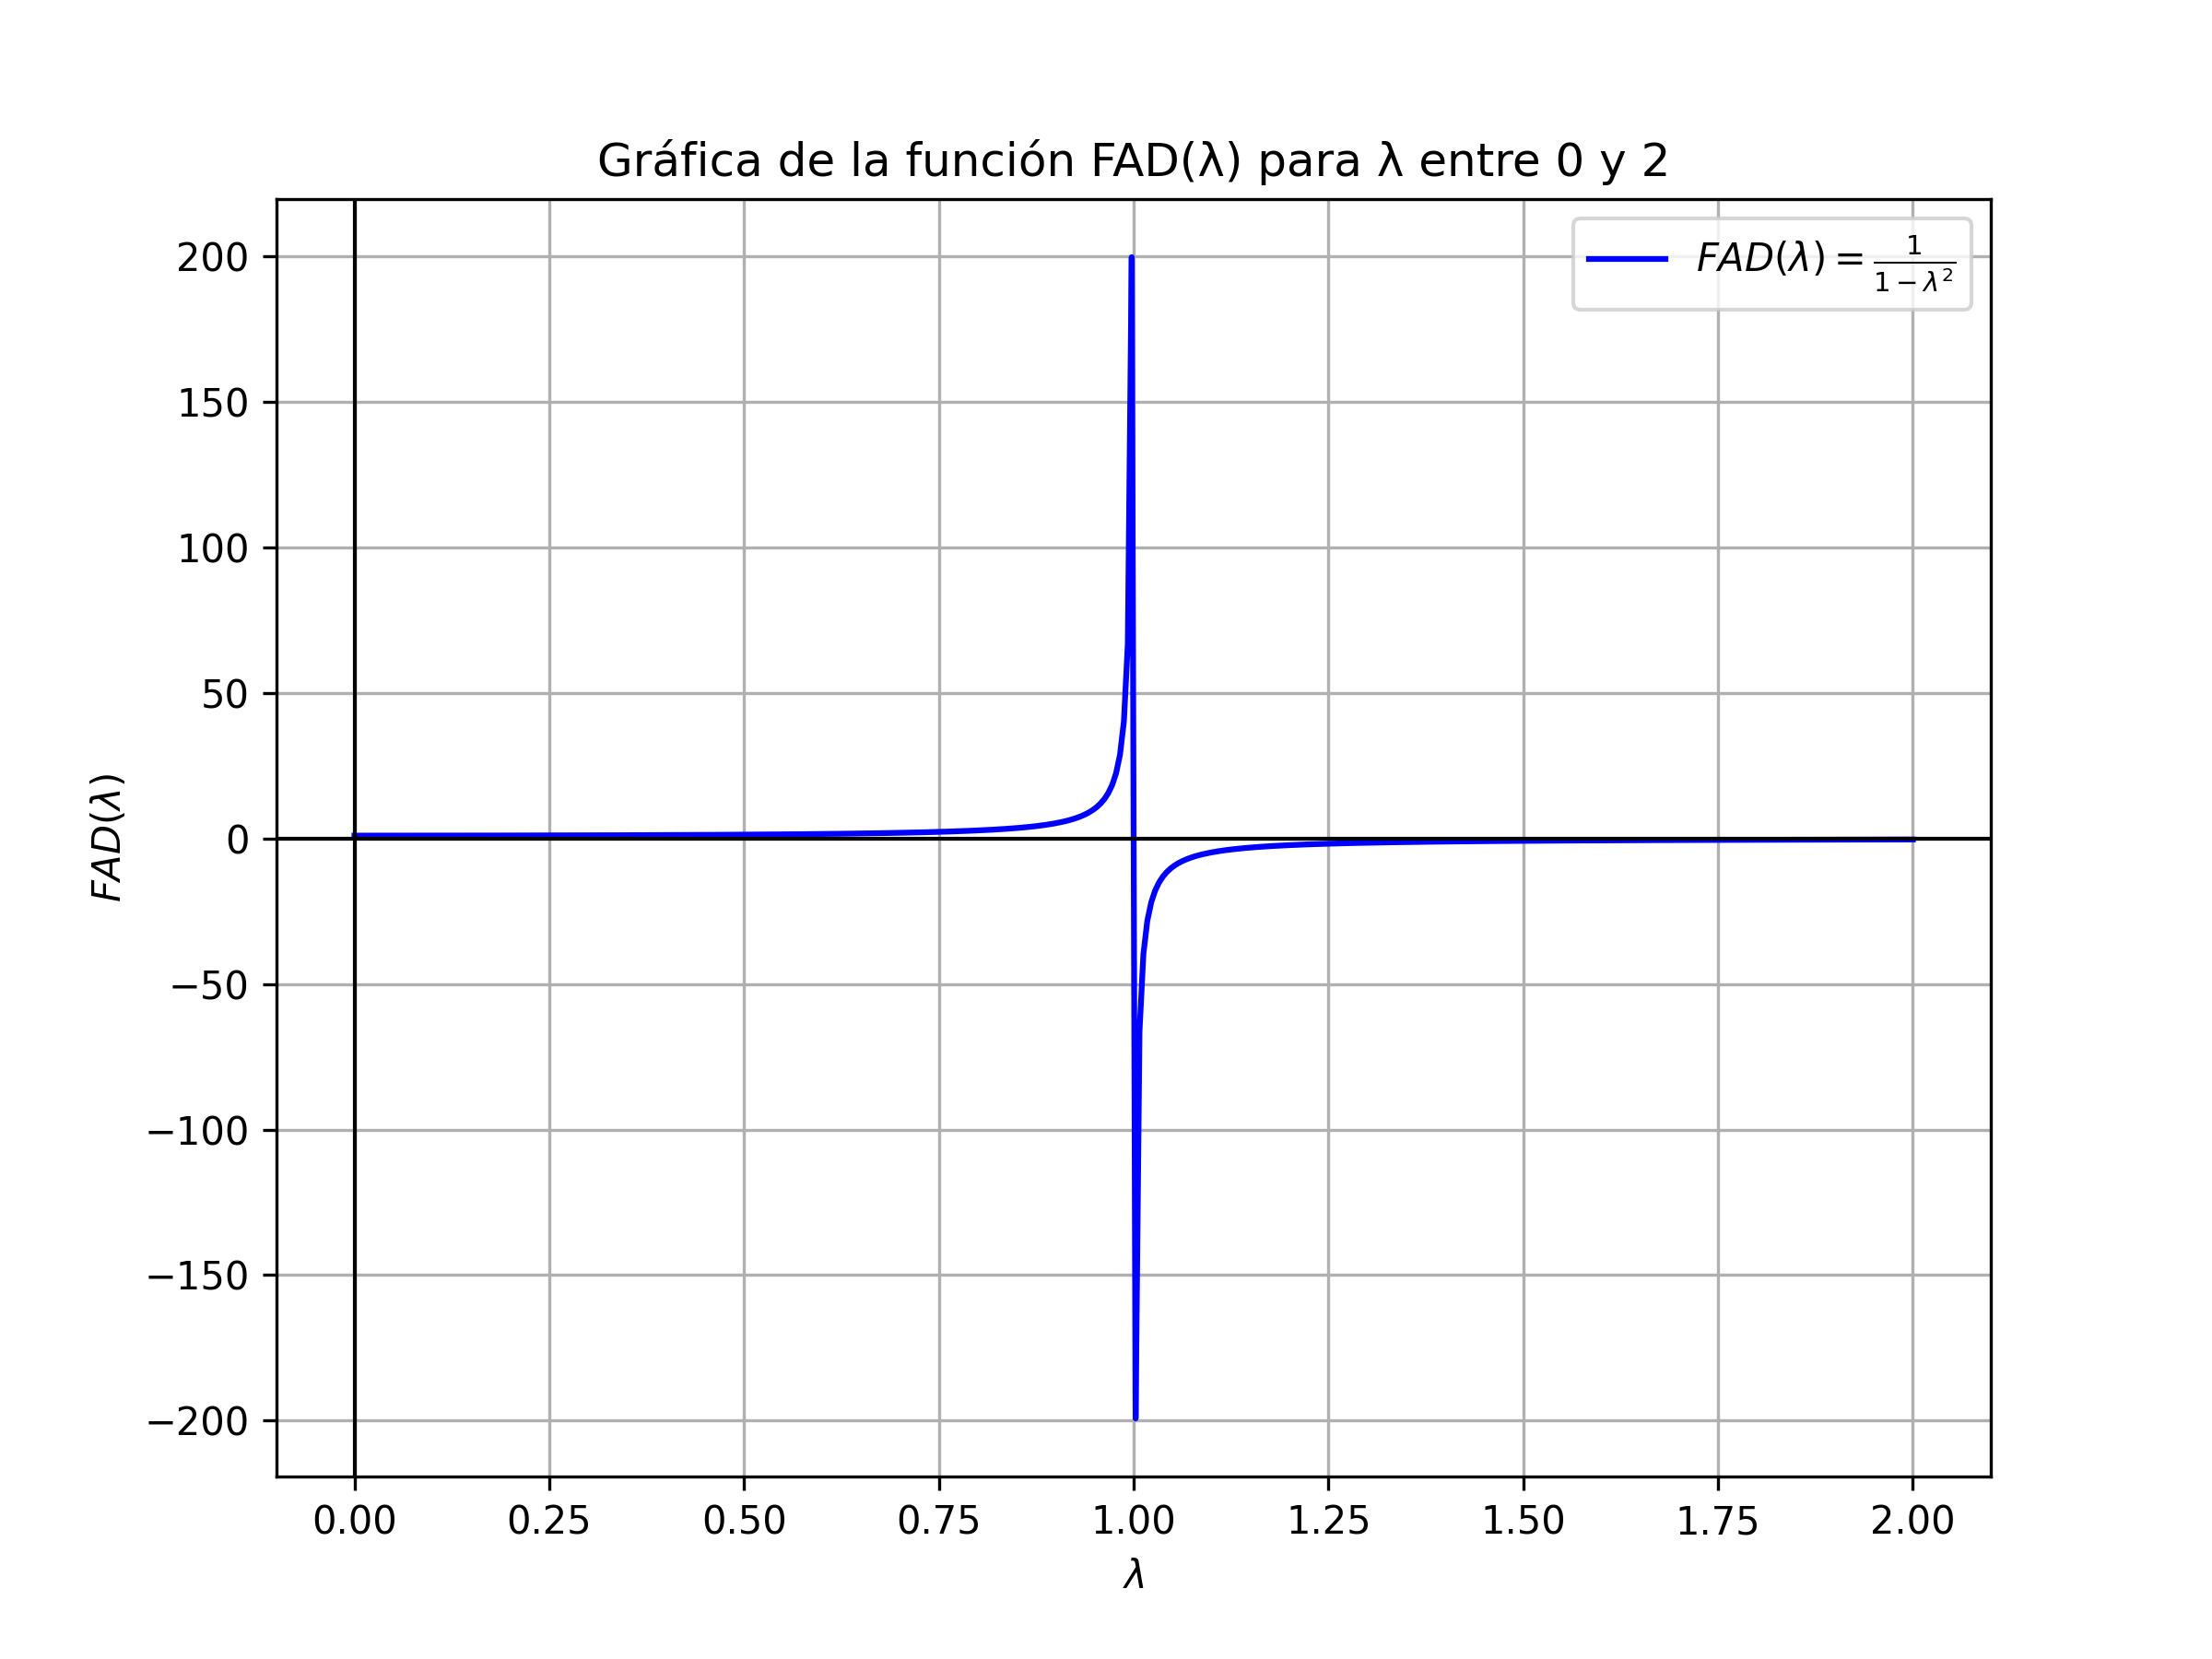
\includegraphics[width=0.6\textwidth]{GRAFICOS/FAD.png}
    \caption{FAD segun $\lambda$}
    \label{fig:ejemplo1}
\end{figure}

\section{Armortiguadores y resortes en linea}

Para calcular el valor $c_\theta$ o $k_\theta$, se deben hacer dos equilibrios de momento, uno para el desplazamiento y otro para la rotacion:

Se tiene el siguiente caso ejemplo:

Rotacion (no depende del centro de gravedad, sino del centroide)

\begin{equation}
    M_{rot} = \bar{\alpha}\cdot \dot{\theta}\cdot \frac{L}{2}\cdot \frac{L}{2}\cdot \frac{1}{2}\cdot \frac{2}{3}\cdot \frac{L}{2} \cdot 2 \rightarrow \alpha_{\theta 1} = \frac{\bar{c} \dot{\theta} L^3}{12}
\end{equation}

Lineal (depende del centro de gravedad y centroide)

\begin{equation}
    M_{lin} = \dot{\alpha} \cdot L \cdot cg \cdot \dot{\theta} \cdot cg \rightarrow \alpha_{\theta 2} = \bar{\alpha} \cdot L \cdot cg^2
\end{equation}



\end{document}
